%%%%%%%%%%%%%%%%%%%%%%%%%%%%%%%%%%%%%%%%%%%%%%%%%%%%%%%%%%%
% EPFL report package, main thesis file
% Goal: provide formatting for theses and project reports
% Author: Mathias Payer <mathias.payer@epfl.ch>
%
% This work may be distributed and/or modified under the
% conditions of the LaTeX Project Public License, either version 1.3
% of this license or (at your option) any later version.
% The latest version of this license is in
%   http://www.latex-project.org/lppl.txt
%
%%%%%%%%%%%%%%%%%%%%%%%%%%%%%%%%%%%%%%%%%%%%%%%%%%%%%%%%%%%
\documentclass[a4paper,11pt,oneside,MScThesis]{report}
% Options: MScThesis, BScThesis, MScProject, BScProject
\usepackage[MScThesis,lablogo]{EPFLreport}
\usepackage{xspace}

\title{Exploring Cepheid variables periodicities using novel distance-correlation based periodograms}
\author{Kent Barbey}
\supervisor{Giordano Viviani}
\adviser{Richard Irving Anderson}
%\coadviser{Second Adviser}
\expert{Xavier Dumusque}

\newcommand{\sysname}{FooSystem\xspace}
\begin{document}
\maketitle
\dedication{\textbf{Pumbaa}: Hey, Timon, ever wonder what those sparkly dots are up there? \\

\textbf{Timon}: Pumbaa, I don’t wonder, I know.\\

\textbf{Pumbaa}: Oh. What are they?\\

\textbf{Timon}: They’re fireflies. Fireflies that, uh… got stuck up on that big bluish-black thing.\\

\textbf{Pumbaa}: Oh, gee. I always thought they were balls of gas burning billions of miles away.\\

\textbf{Timon}: Pumbaa, with you, everything’s gas.\\

    --- \textit{The Lion King}\\}
\makededication
\acknowledgments{\vspace{0.5cm}thanks}

\makeacks
\newpage
\chapter*{Acronyms \& Abbreviations}
\begin{acronym}
    \acro{GCVS}{General Catalogue of Variable Stars}
    \acro{GLS}{Generalised Lomb-Scargle Periodogram}
    \acro{PDC}{Partial Distance Correlation}
    \acro{PLR}{Period-Luminosity Relation}
    \acro{RV}{Radial Velocity}
    \acro{SB1}{Single-lined Spectroscopic Binaries}
    \acro{SPARTA}{\textbf{SP}ectroscopic v\textbf{AR}iabili\textbf{T}y \textbf{A}nalysis}
    \acro{STIS}{Space Telescope Imaging Spectrograph}
    % \acro{alfUMi}{$\alpha$ Ursae Minoris}
    \acro{delCep}{$\delta$ Cephei}
    \acro{zetGem}{$\zeta$ Geminorum}
\end{acronym}
\newpage
\begin{abstract}
blablabla
\end{abstract}

\maketoc
%%%%%%%%%%%%%%%%%%%%%%
\chapter{Introduction}
    \section{Brief historical context}
    \label{historical_context}
Among the astronomical revolutions that occurred during the XVI and early XVII centuries, the realisation that the sky was not eternally invariable as Aristotle had taught (\textit{On the Heavens}, 350 B.C.) for almost two millennia stands a special place. Indeed, the first variable star, \textit{Mira}, was identified in 1596 by David Fabricius\footnote{It is worth mentioning that the variability of stars such as \textit{Algol} and \textit{Mira} had been described as early as 3200 years ago in many different societies but these observations were at best circumstantial \parencite{Wilk1995MythologicalStars}.}. Its brightness oscillating between 2 and 5 [mag]. Around the same time in 1572 and 1604, supernovae were observed and described, thus putting an end to the myth. It is however only two centuries later, in 1784, that John Goodricke suggested the first correct explanation to the variability  of a star, \textit{Algol}, an eclipsing binary. Finding the right cause to the variability of a star is a delicate endeavour as many effects, different in substance but similar in form, can cause it. This led and still leads to wrong interpretations of variability e.g. when \textit{intrinsically} (see \textbf{Sec.} \ref{cepheids_intro}) varying stars are misclassified as eclipsing binaries.

\noindent Since then, the number of variable stars has increased tremendously in particular with the advent of photography in the first half of the XVIII century. Nowadays, almost 60'000 variable stars are listed in the \href{https://heasarc.gsfc.nasa.gov/w3browse/all/gcvs.html}{\textit{\ac{GCVS}}} and new ones are discovered every year with the recent development of large-scale surveys\parencite{Eyer2007VariableDiagram}.

\noindent Variable stars and more generally time variability play a crucial role in astronomy. The diversity of variable phenomena observable on human timescales is also significant as \textbf{Fig.} \ref{1a} suggests\footnote{This \textit{variability tree} is essentially photometric oriented.} but they can be classified in two large categories: extrinsic and intrinsic variability. The former comprises phenomena where the brightness change (light curve variability) is caused by geometrical effects such as an object eclipsing another one or bending its light (gravitational lensing) whereas the latter includes objects where the light curve variability is due to physical changes in the object itself. The intrinsic variability category includes an interesting subcategory: regularly pulsating stars (to which \textit{Mira} belong to) and more specifically: Cepheids.

%%%%%%%%%%%%%%%%%%%%%%
            \section{Cepheids and their periodicities}
            \label{cepheids_intro}
            Classical cepheids, named after their prototype $\delta$ Cephei, are late-type (super)-giant stars that maintain stable radial pulsation on periods of 2 to 70 days for the ones belonging to the Milky Way\parencite{Eyer2007VariableDiagram}. A brief overview of the phenomenon is given in \textbf{Sec.} \ref{stellar_pulsations}. Cepheids have played a crucial role in a broad range of astrophysical topics ranging from cosmology to stellar physics. Indeed, upon the discovery of the \ac{PLR} of Cepheids by Leavitt \& Pickering (1912), astrophysics had found its first \textit{standard candle} to measure distances to faraway galaxies and eventually deduce the present expansion rate of the universe $H_0$ called the \textit{Hubble constant}. On another hand, Cepheids are invaluable natural laboratories for testing stellar evolution theory.
            
    
            \begin{figure}[H]
            \centering
            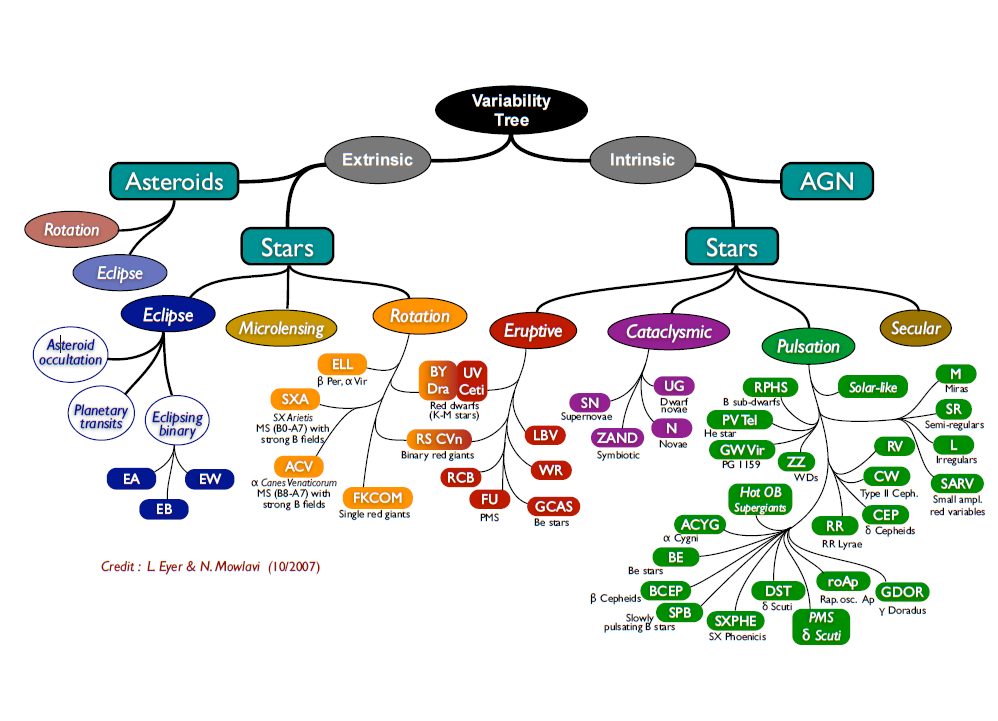
\includegraphics[width=0.99\textwidth]{report/images/variability_tree.png}
            \caption{Photometric variability tree of astrophysical phenomena observable in our universe from \cite{Eyer2007VariableDiagram}. The first division distinguishes between intrinsic and extrinsic variability. The second one between the type of object considered. The third level identifies the origin of the variability. Finally, the last division groups objects of either similar photometric behaviour or similar physical characteristics.}
            \label{1a}
            \end{figure}

            \noindent The intrinsic variability periods of Cepheids can be found spectroscopically and photometrically, both agreeing to high-precision thus indicating a common cause to the phenomenon and partially solving the problem of misclassification mentioned above. Spectroscopically, these intrinsic variations appear as a combination of shape and shift variability of the spectrum's features over time. However, many Cepheids have been confirmed to be part of multiple star systems and a majority (at least 60\%) are believed to be in such systems (Szabados, 2003). These \textit{binary Cepheids} are in most cases \ac{SB1}. On a more recent note, most stars if not all, are believed to host planets. These gravitational companions, stars or planets, appear in the star's spectrum as Doppler shift variations which are encapsulated in the \ac{RV} curve of the star.

            \noindent \ac{RV}s are however the reduction to a single number of the consequent information a spectrum contains. They therefore have to be manipulated and interpreted accordingly. The emergence of high-precision velocimetry observations, related to the discovery of the first exoplanet around a solar-type star(M. Mayor \& D. Queloz, 1995), has led to the discovery of many companions, stars and planets alike, to non-variable and variable stars. As hinted in \textbf{Sec.} \ref{historical_context}, the misinterpretation of \ac{RV} variations being due to an orbital companion is still an ongoing issue especially around variable stars where strong stellar activity can mimic orbital signals. Recent and less recent examples are the challenged discoveries of companions around Barnard's star \parencite{Lubin2021StellarPositive}, HD 200466 \parencite{Carolo2014A200466} and HD 166435 \parencite{Queloz2001No166435,Queloz2001No166435b}. Conversely, orbital signals introduce deviation in the \ac{RV} curve and the unknown presence of a bright companion brings in parasitic flux to the light interpreted to be emitted from the star alone thus hindering the efforts into correctly characterising these objects and calibrating subsequent models and relations such as the \ac{PLR}\parencite{Anderson2009ClassicalRotation}. Furthermore, \ac{RV}s can be considered a nuisance parameter in the paradigm of stellar classification where they should be discounted from the spectra in order to compare them on a common wavelength grid (Katz et al. 1998).

            \noindent On a stellar evolution note, studying \ac{SB1} Cepheids is of important matter for a handful of good reasons (see \cite{Anderson2009ClassicalRotation} \textbf{Sec.} 2.2 for more details) among which the famous \textit{mass discrepancy problem} of Cepheids. Masses determined using standard stellar evolution models are larger to as much as 20\% than masses determined using pulsation modelling or orbital dynamics of a companion \parencite{Guzik2021ChallengesModeling}. Given the vast proportion of suspected \ac{SB1}s, studying them is an ingredient to solving this issue.
            %citer guzik
    %%% DONT FORGET TO SAY THAT YOUR CODE CAN FIND PERIODICITIES THAT GLS DOESN?T FIND SUCH AS BG CRU SECOND MODE(Find others?)
    \section{Outlines of this work}

       In recent years, numerous methods have been developed to reduce or predict the impact of stellar activity on orbital signals from \ac{RV} curves deduced from stellar spectrum e.g. \cite{DeBeurs2022IdentifyingNetworks, Aigrain2012APhotometry, Bellotti2022MitigatingSelection}. Conversely, efforts have been made to uncover the causes and effects of the presence of orbital companions on stellar evolution models and observations of Cepheids.

       \noindent This thesis is an exploratory work of such a promising new method developed in \cite{Binnenfeld2021NewVariation} that was built upon \parencite{Binnenfeld2020USuRPER:Spectra} and (Zucker 2015, 2016, 2018, 2019). The capabilities and shortcomings of this period-finding method are investigated and preliminary results are presented on a dataset of 15 objects.
       
       \noindent This method is based on the statistical notion of distance correlation \parencite{Szekely2007MeasuringDistances} and \ac{PDC} \parencite{Szekely2014PartialDissimilarities} and effectively helps in distinguishing spectral shape variability from orbital radial velocities by limiting the nuisance induced from one to the other and eventually finding periodicities. One of the advantages being that, contrary to other methods cited above, both signals are supposedly improved thus exploiting better the information contained in a star's varying spectrum. The algorithm has been implemented into a public \texttt{Python} package, \href{https://github.com/SPARTA-dev/SPARTA/tree/master}{\texttt{\ac{SPARTA}}}, on which this work is based.

       \noindent The structure of the thesis is as follows. \textbf{Sec.} \ref{theory} lays the mathematical and physical foundations necessary to understand the ins and outs of the method and the results. First, the nature of the data manipulated, stellar spectra and \ac{RV}s, is briefly described. Then a small review on Cepheids and their periodicities is given. In \textbf{Sec.} \ref{finding_periods} the different period-finding techniques are summarised with an accent being made on Fourier-based methods and especially the \ac{GLS}. Finally, the distance correlation-based periodogram used throughout this work is introduced with first the statistical framework followed by a didactic example replicated from \cite{Binnenfeld2021NewVariation}.

       \noindent \textbf{Sec.} \ref{methods} describes the methodology used. This comprises the instruments, the data acquisition and treatment before feeding it to the periodogram-building algorithm and finally the proper peak analysis.

       \noindent This being an investigation work on a method not yet fully tested, the results are presented in two parts. In \textbf{Sec.} \ref{resultsa}, the different shortcomings and encountered limits of the method are scrutinised. In \textbf{Sec.} \ref{resultsb}, preliminary results on fifteen Cepheids data taken from three different instruments are presented and discussed.

       \noindent Finally, \textbf{Sec.} \ref{future} and \ref{conclusion} give an outlook on the results presented here and the future work to be done to hopefully completely uncover the potential of this new technique.

       

    %say the good reasons to study periodicities of cepheids(at least 3) and state why today's knowledge is lacking. Say what's done in one or two brief sentences and what it improves. Outlines section by section.
%%%%%%%%%%%%%%%%%%%%
\chapter{Mathematical and Physical Foundations}
\label{theory}
%%%%%%%%%%%%%%%%%%%%
    \section{Stellar spectra}
    Quoting \cite{Hearnshaw2014TheStarlight}: 
    
    \noindent \guillemotleft \textit{A spectrum can be regarded as a one-dimensional image in which the intensity of light} (flux) \textit{can be analysed as a function of wavelength.} \guillemotright 

    \noindent All objects interacting electromagnetically possess a spectrum. Stellar spectra represent the energy emitted by a star at given light wavelengths. They are formed by the decomposition of the light received from the star into the different energies contained by its photons using special instruments called \textit{spectrographs} (see \textbf{Sec.} \ref{methods}.1 for a summary. Stellar spectra contain information about a star's temperature, chemical composition, intrinsic luminosity etc... With the right tools, they can also,to some extent, help understand a star's internal and orbital dynamics.
    
    \begin{figure}[H]
        \centering
        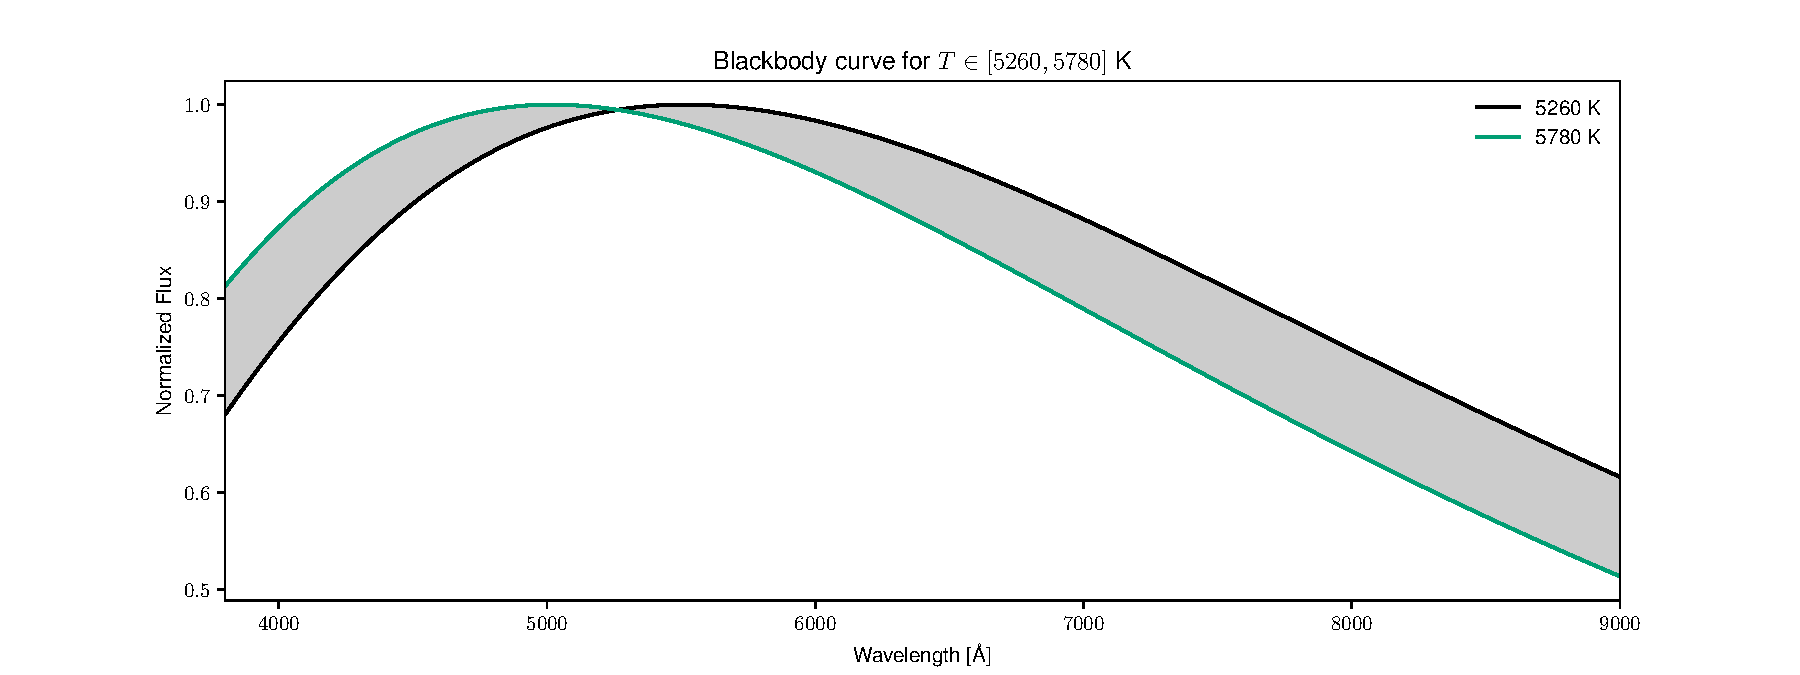
\includegraphics[width=\textwidth]{report/images/chap2_foundations/blackbody_zetgem.pdf}
        \caption{Normalised blackbody curves for temperatures between 5260-5780 [K] and wavelengths ranging from 3800-9000 \AA. }
        \label{2.1a}
    \end{figure}
    % \footnote{Proposal ID: 9786}
    \begin{figure}[H]
        \centering
        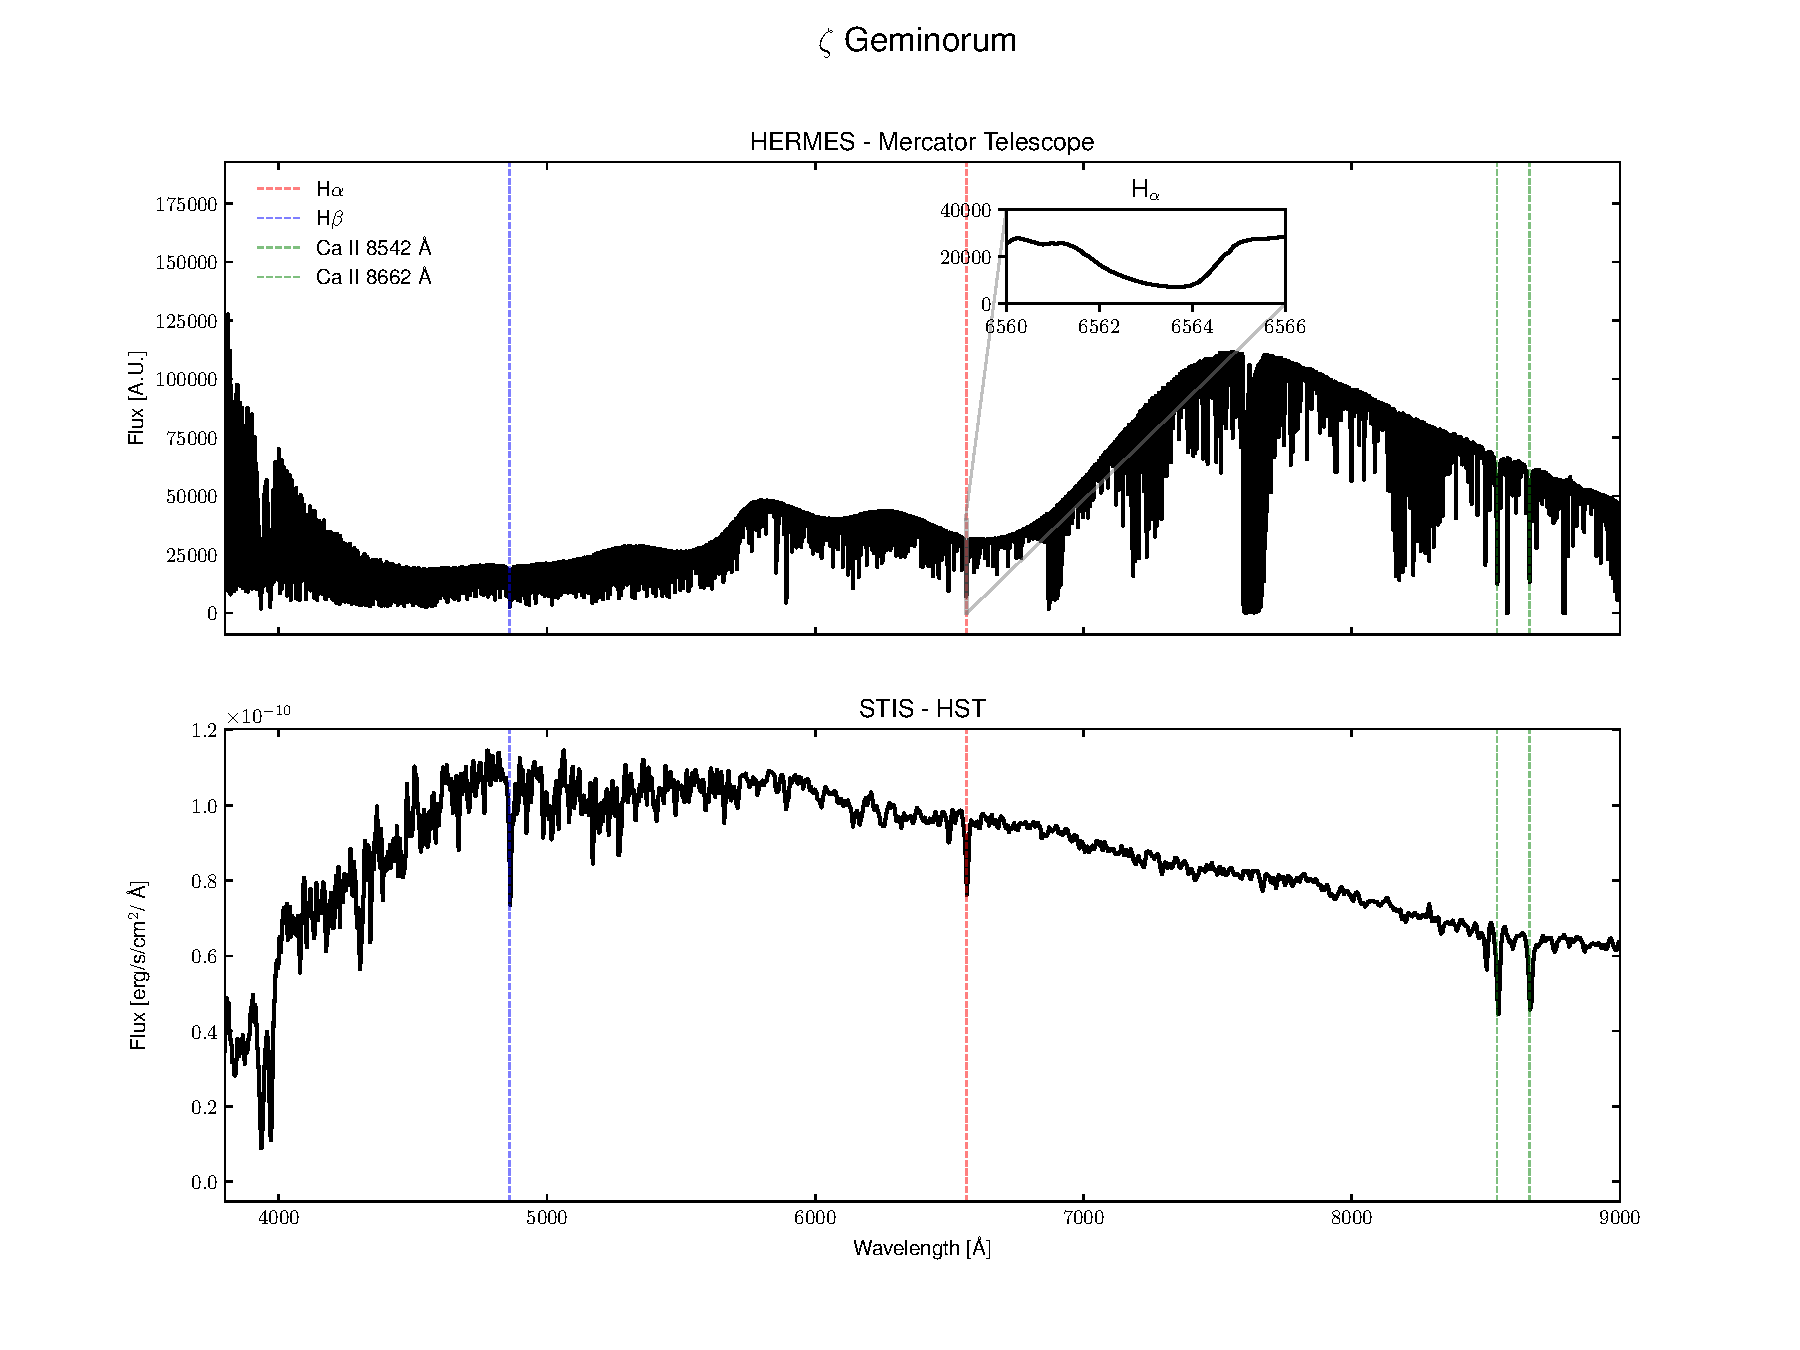
\includegraphics[width=\textwidth]{report/images/chap2_foundations/zetgem_hermes_hst.pdf}
        \caption{(top) Unprocessed merged 1D stellar spectrum of \ac{zetGem} taken by the HERMES spectrograph on the Mercator Telescope at La Palma Observatory on the 26.10.2015. The inset pictures the $H_{\alpha}$ absorption line. (bottom) Spectrum of \ac{zetGem} obtained from the \ac{STIS} instrument aboard the Hubble Space Telescope on the 26.12.2006 and retrieved from the \href{https://mast.stsci.edu/portal/Mashup/Clients/Mast/Portal.html}{MAST Archive} . Notice the resolution difference between both spectrographs and more importantly the influence of Earth's atmosphere on the general shape of HERMES spectrum and the appearance of telluric lines.}
        \label{2.1b}
    \end{figure}
    
    \section{Radial velocities}
        %say that we are looking at metallic lines.
        \begin{figure}[H]
        \centering
        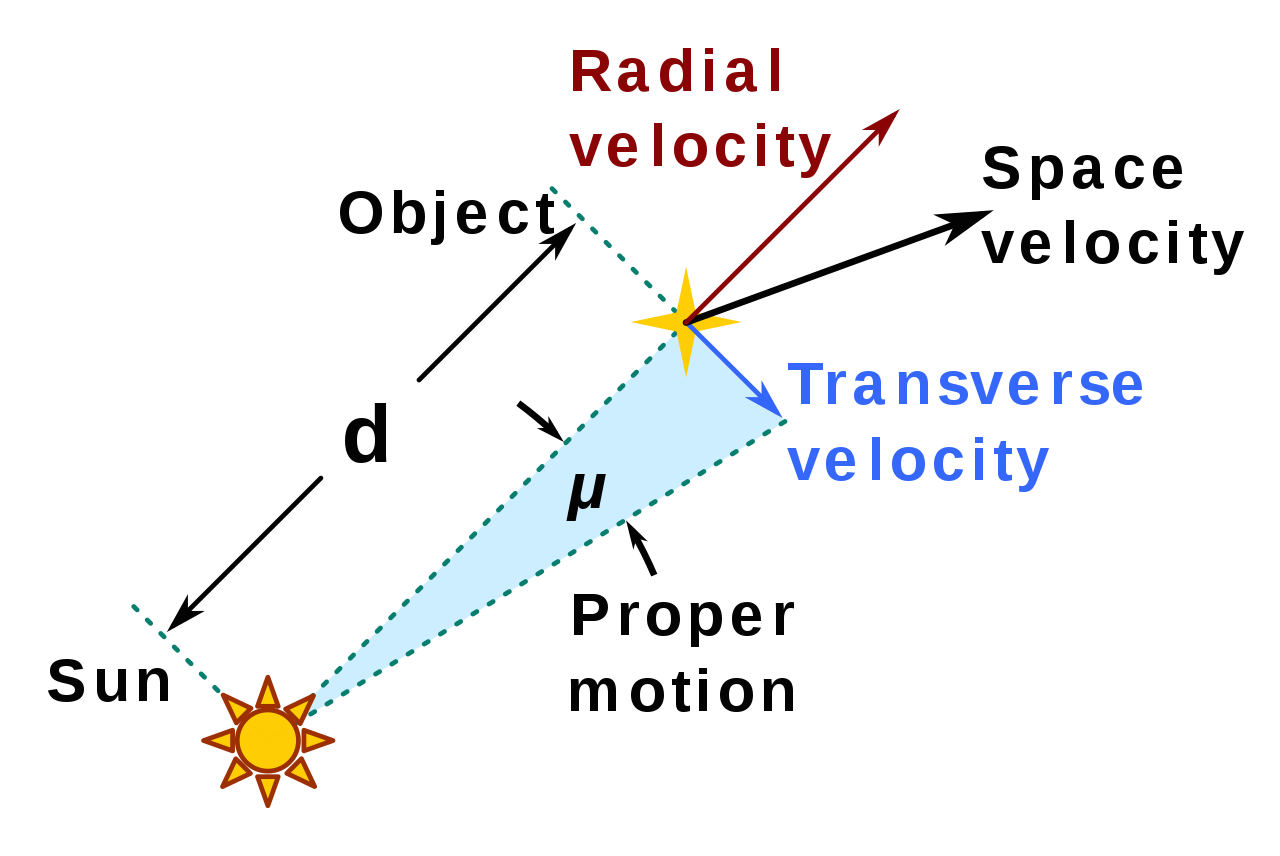
\includegraphics[width=0.6\textwidth]{report/images/chap2_foundations/1280px-Proper_motion.svg.png}
        \caption{Caption}
        \label{2.2a}
        \end{figure}

        \begin{figure}[H]
        \centering
        \begin{subfigure}{.45\textwidth}
            \centering
            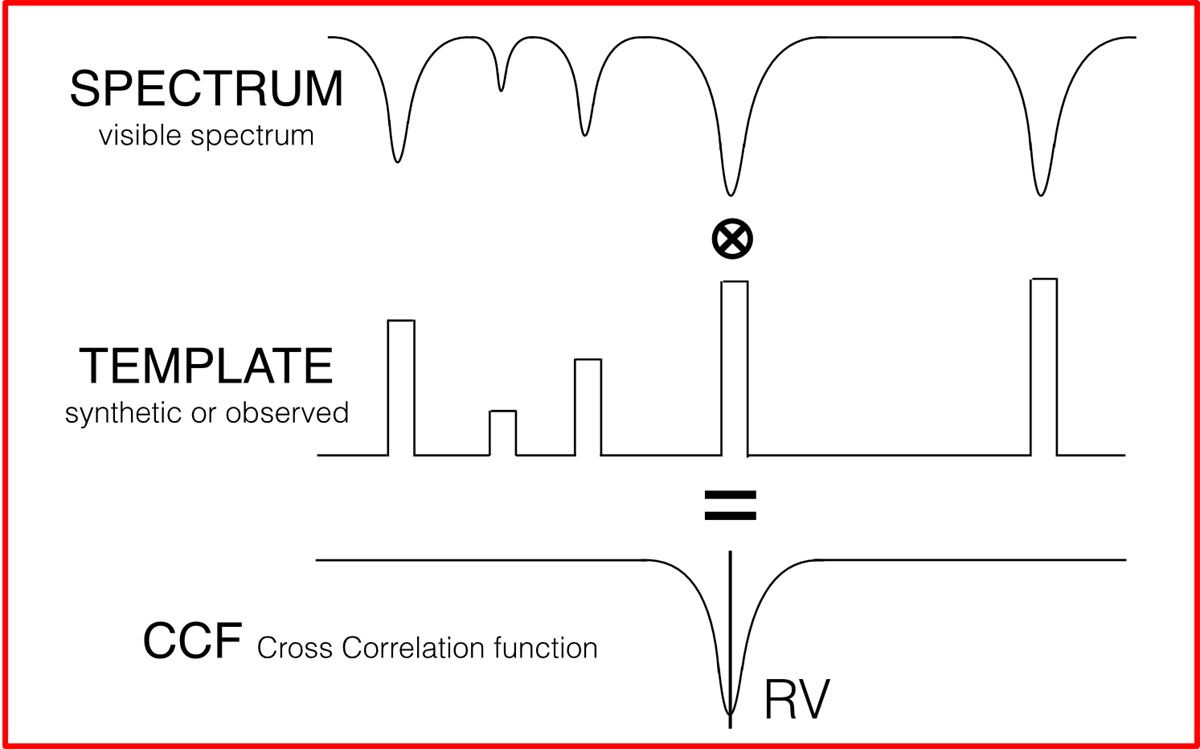
\includegraphics[width=\textwidth]{report/images/chap2_foundations/ccf_template.png}
        \end{subfigure}%
        \hspace{1em}
        \begin{subfigure}{.45\textwidth}
            \centering
            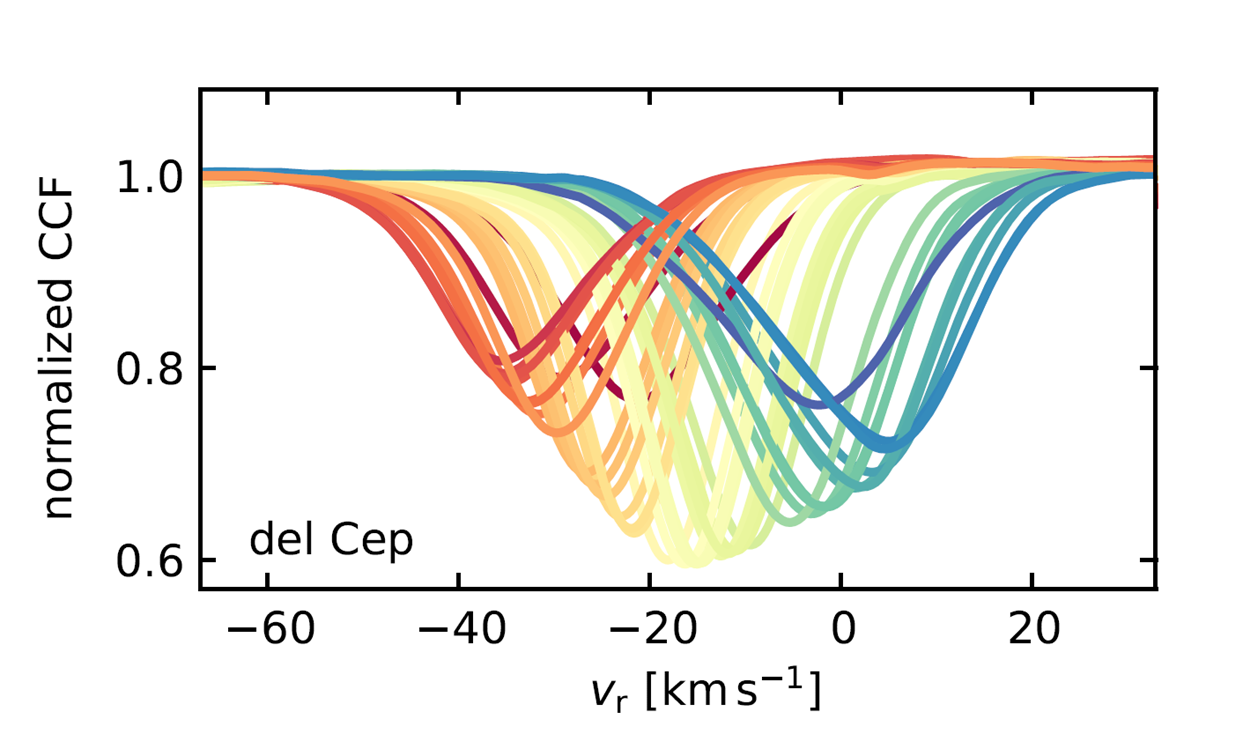
\includegraphics[width=\textwidth]{report/images/chap2_foundations/delCep_ccf.png}
        \end{subfigure}
        \caption{\ac{delCep}}
        \label{2.2b}
        \end{figure}

        \begin{figure}[H]
        \centering
        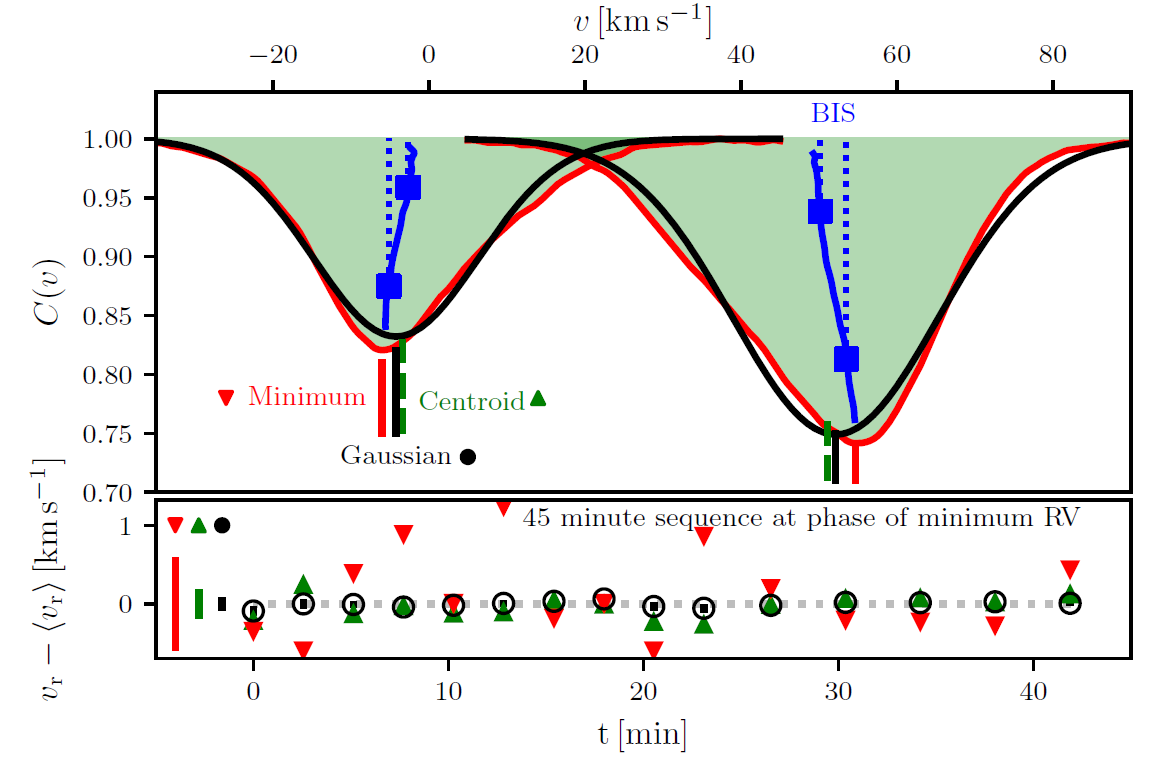
\includegraphics[width=0.8\textwidth]{report/images/chap2_foundations/anderson_2018.png}
        \caption{Caption}
        \label{2bonus}
        \end{figure}

        \begin{figure}[H]
        \centering
        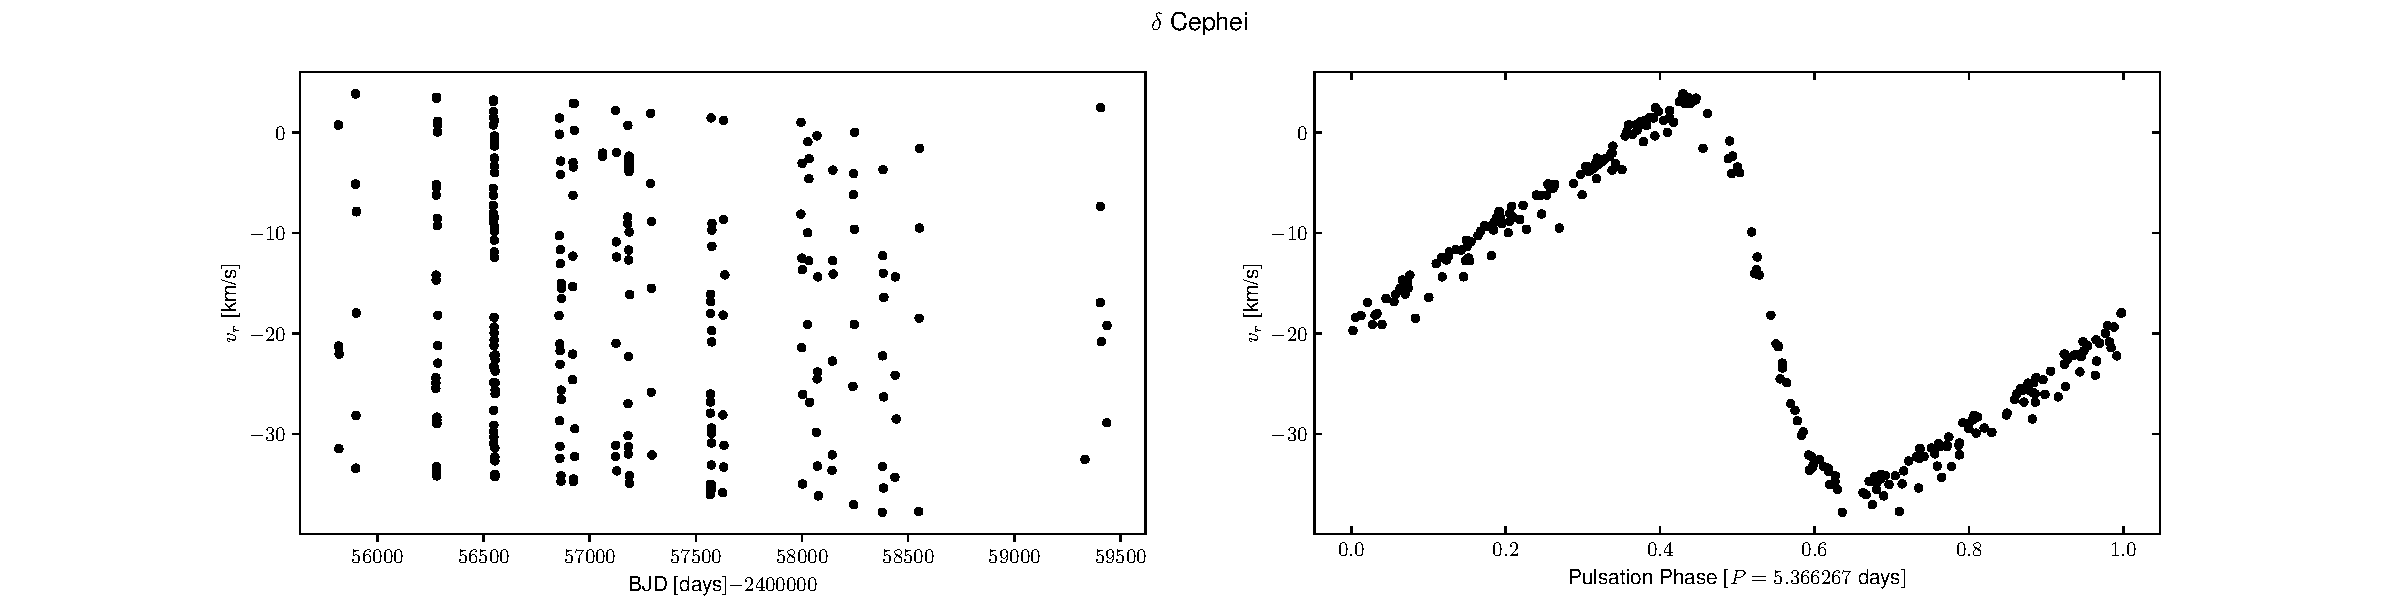
\includegraphics[width=\textwidth]{report/images/chap2_foundations/delcep_rv.pdf}
        \caption{Caption}
        \label{2.2c}
        \end{figure}
    
    \section{Cepheids}
    
        \subsection{Stellar pulsations}
        \label{stellar_pulsations}
        %see chap 2 of anderson, talk also about the three types of cepheids + rrlyr
        \begin{figure}[H]
        \centering
        \begin{subfigure}{.45\textwidth}
            \centering
            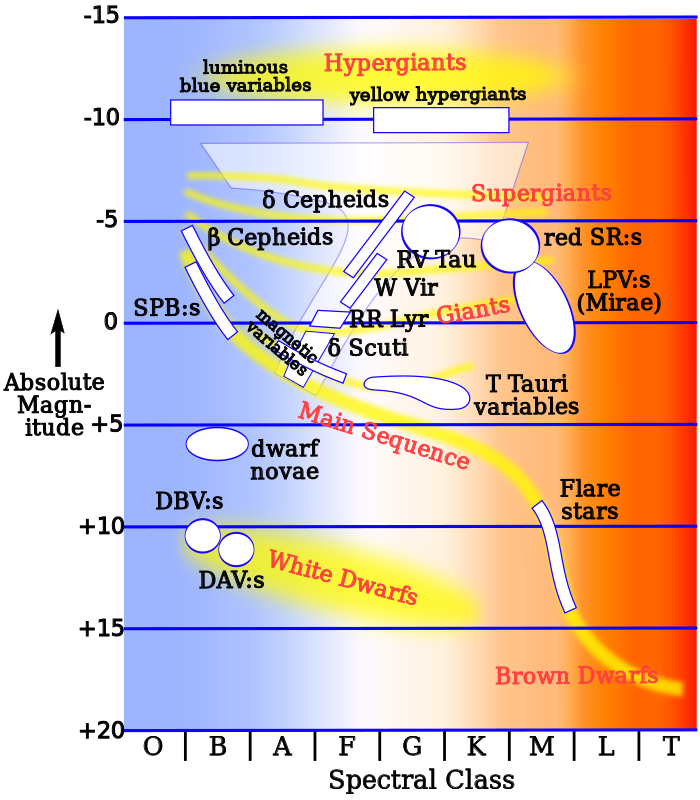
\includegraphics[width=\textwidth]{report/images/chap2_foundations/HR-vartype.png}
        \end{subfigure}%
        \hspace{1em}
        \begin{subfigure}{.45\textwidth}
            \centering
            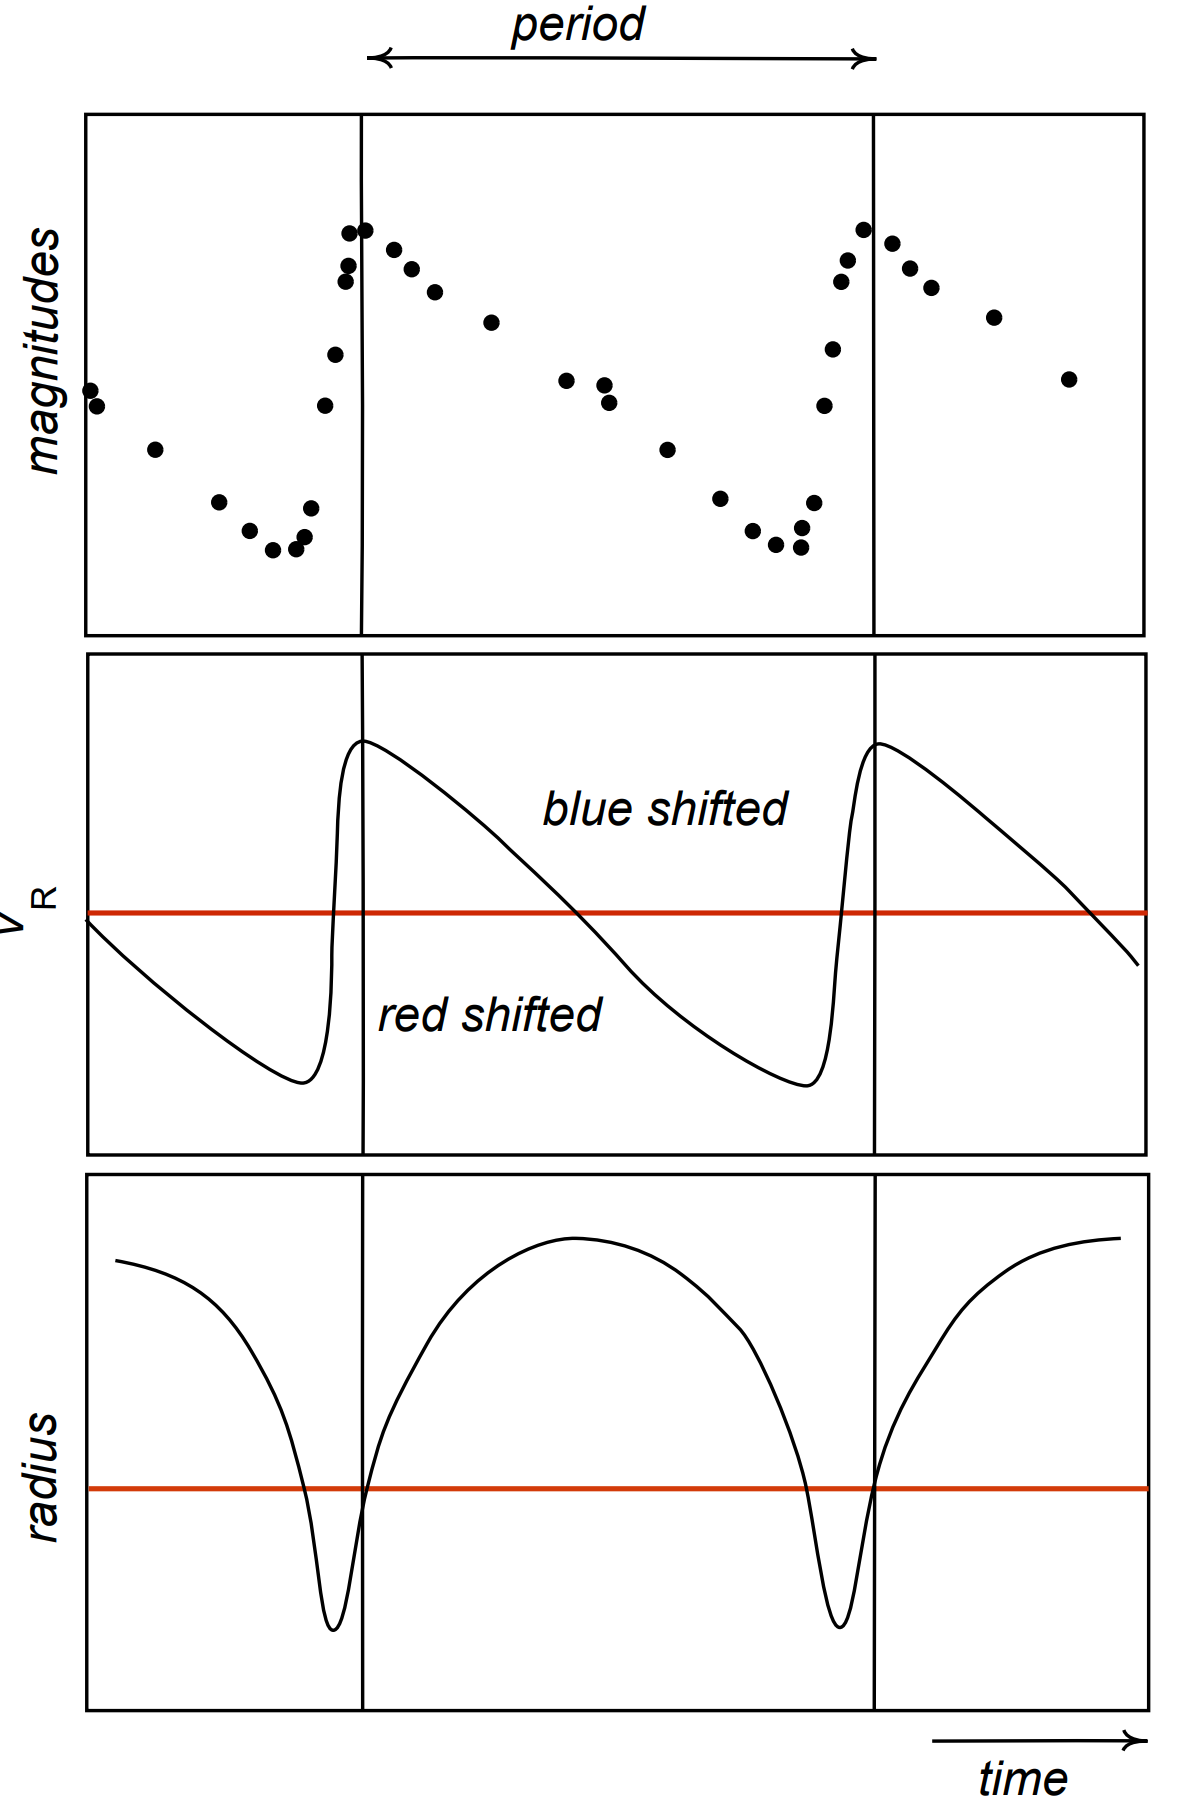
\includegraphics[width=0.79\textwidth]{report/images/chap2_foundations/gautschy_2003.png}
        \end{subfigure}
        \caption{???}
        \label{2.3b}
        \end{figure}
        
        \begin{figure}[H]
        \centering
        \begin{subfigure}{.45\textwidth}
            \centering
            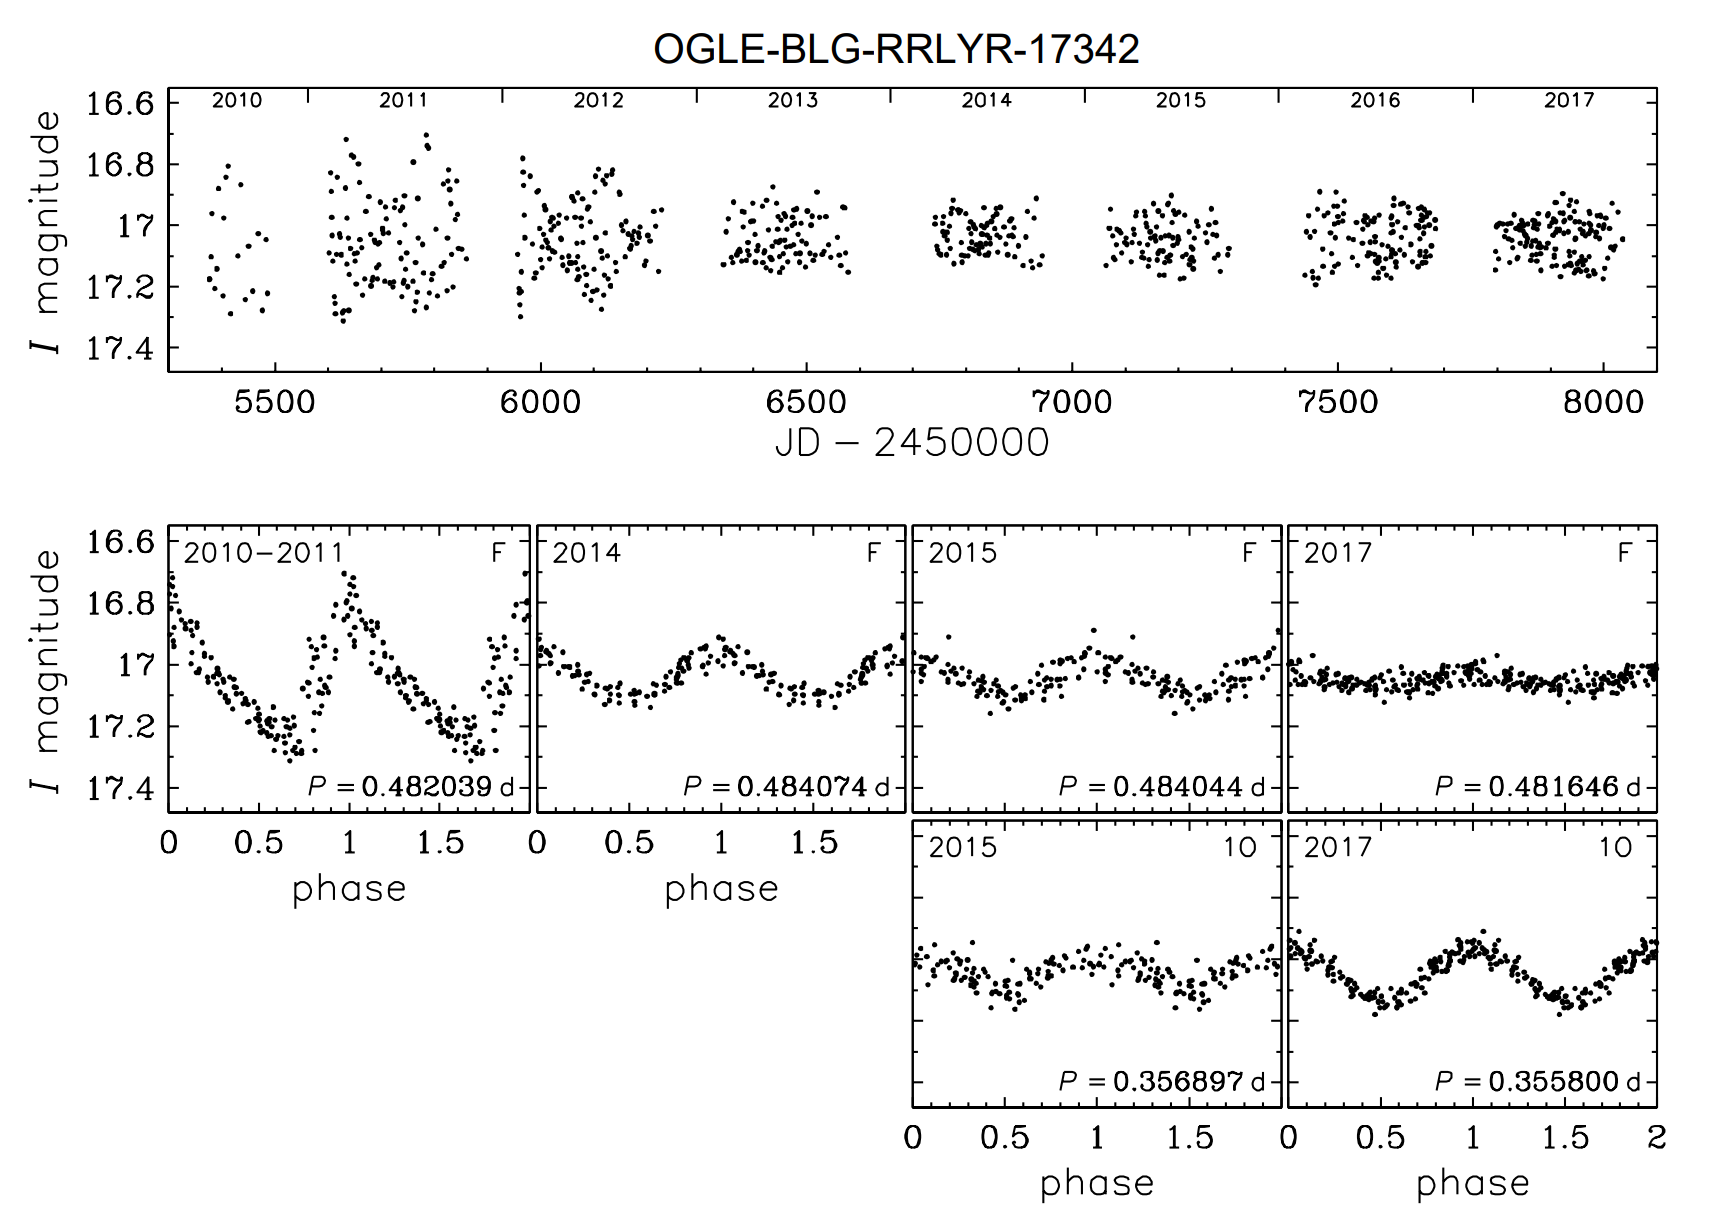
\includegraphics[width=\textwidth]{report/images/chap2_foundations/double_mode.png}
            \vspace{2em}
        \end{subfigure}%
        %\hspace{1em}
        \begin{subfigure}{.45\textwidth}
            \centering
            \includegraphics[width=\textwidth]{report/images/chap2_foundations/spherical_harmonics.png}
        \end{subfigure}
        \caption{???}
        \label{2.3c}
        \end{figure}
        
        \subsection{Cepheid binaries}
        %talk about radial velocity jitter that can be caused by companion(see candidacy exam giordano)
    \section{Finding periodicities}
    \label{finding_periods}
        \subsection{Fourier-based methods}

        
        \begin{figure}[H]
        \centering
        \begin{subfigure}{.45\textwidth}
            \centering
            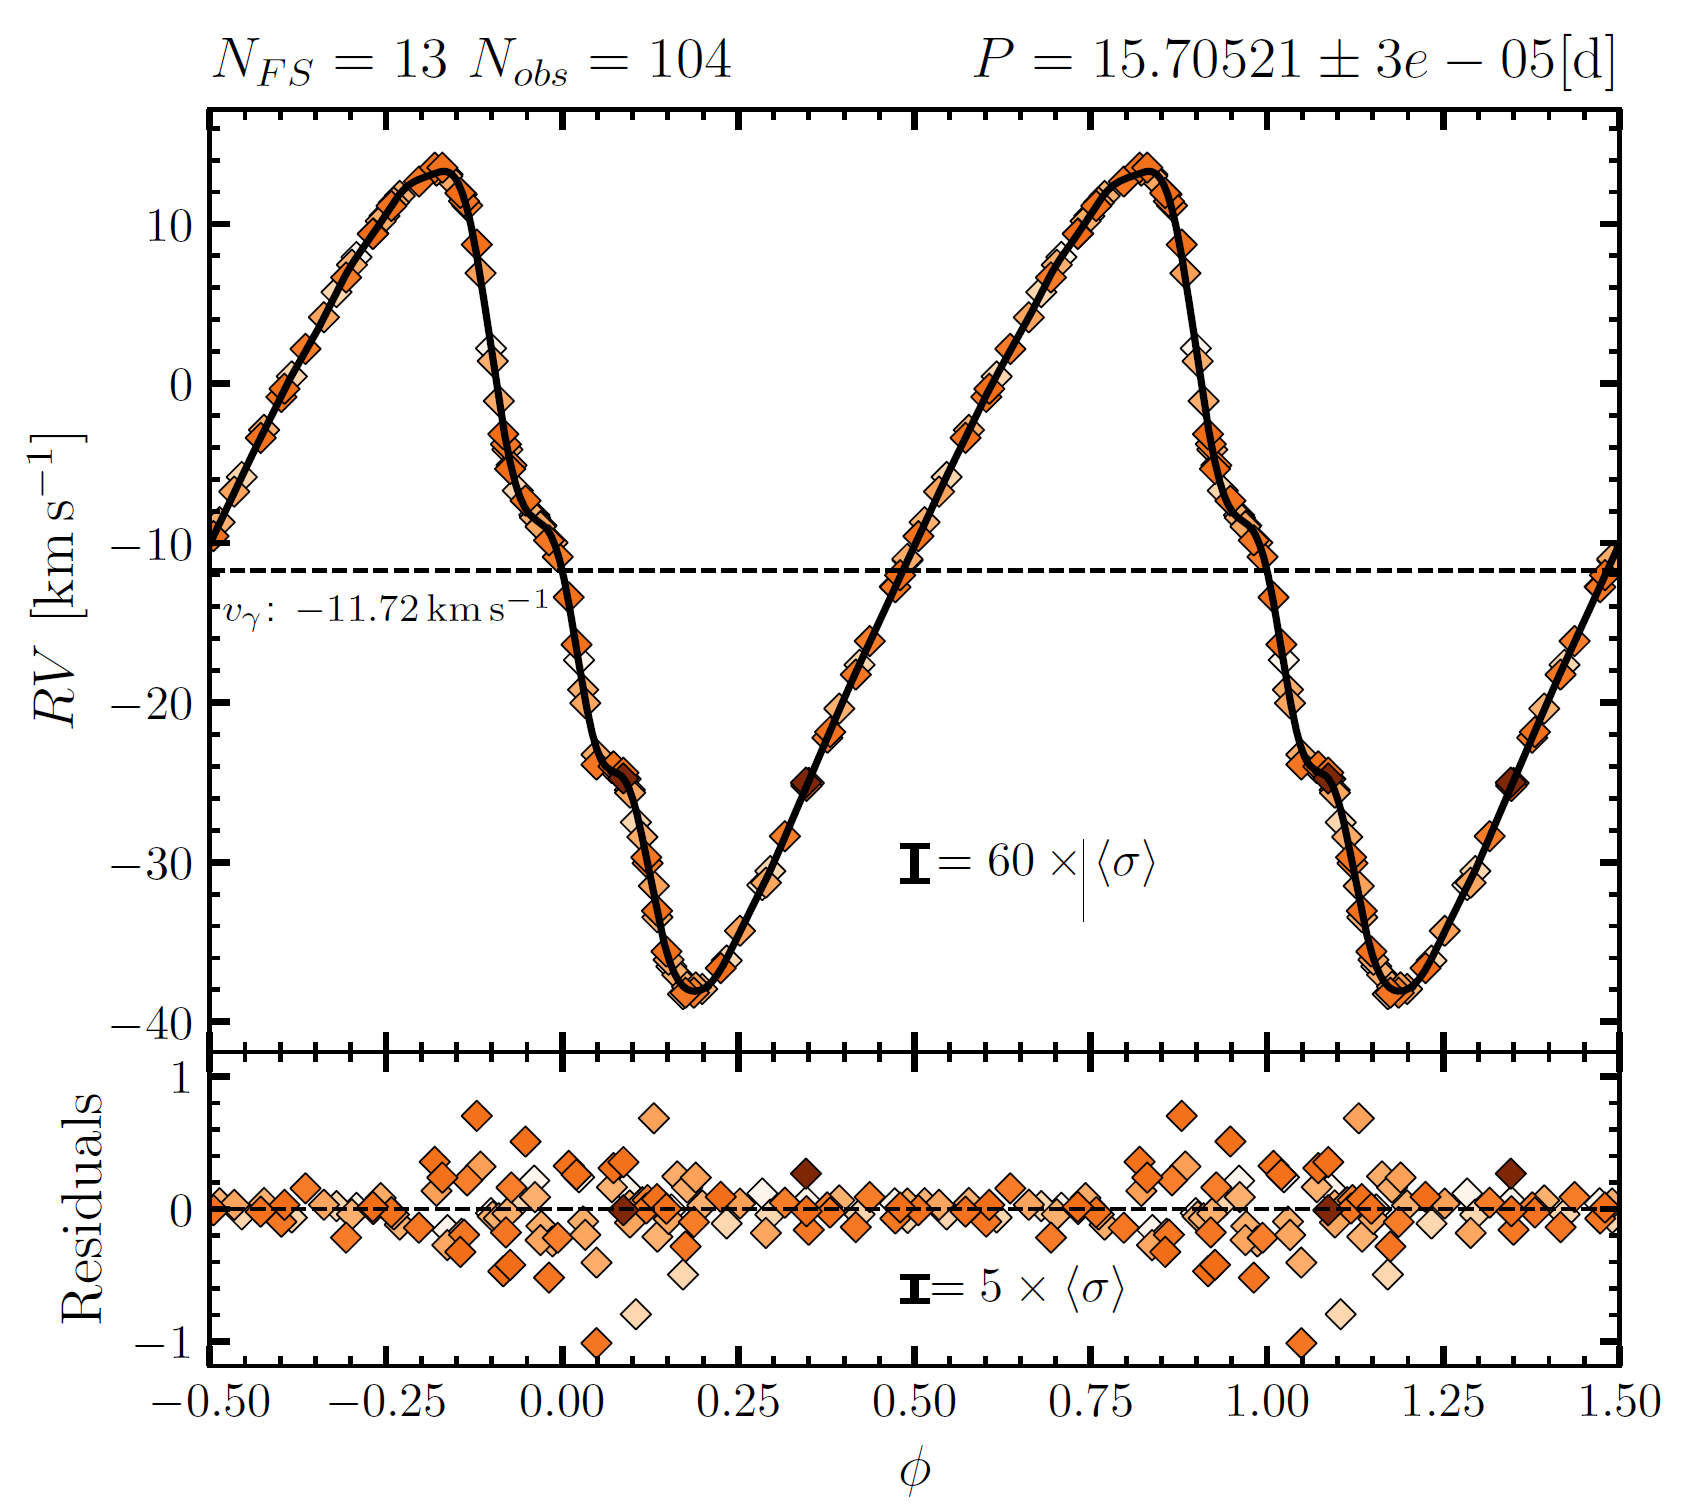
\includegraphics[width=0.8\textwidth]{report/images/chap2_foundations/fourier_fit.png}
            %\vspace{2em}
        \end{subfigure}%
        \hspace{1em}
        \begin{subfigure}{.45\textwidth}
            \centering
            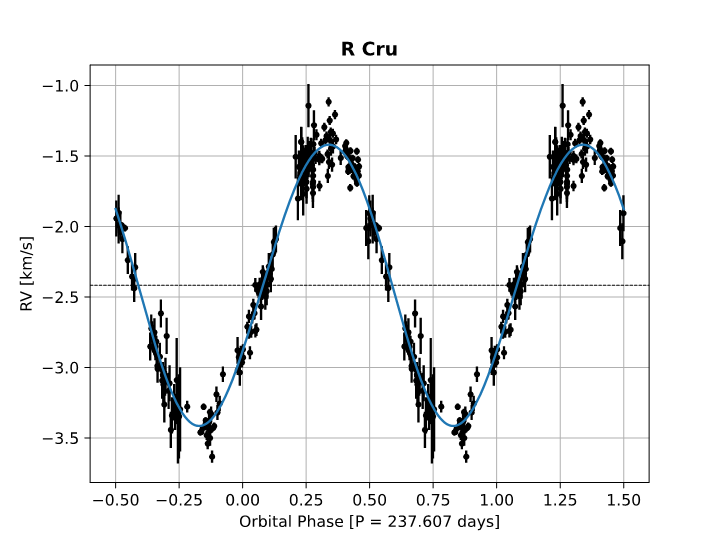
\includegraphics[width=\textwidth]{report/images/chap2_foundations/rcru_orbital.png}
        \end{subfigure}
        \caption{???}
        \label{2.4a}
        \end{figure}
        
            \subsubsection{The Lomb-Scargle periodogram}

            \begin{figure}[H]
            \centering
            \begin{subfigure}{.5\textwidth}
                \centering
                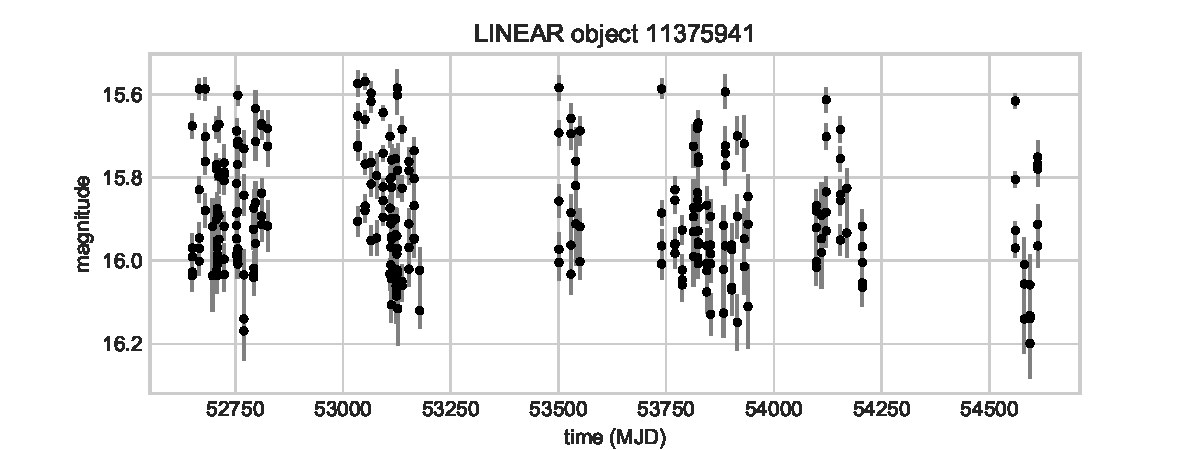
\includegraphics[width=0.88\textwidth]{report/images/chap2_foundations/fig01_LINEAR_data.pdf}
                \vspace{1em}
            \end{subfigure}%
            \begin{subfigure}{.5\textwidth}
                \centering
                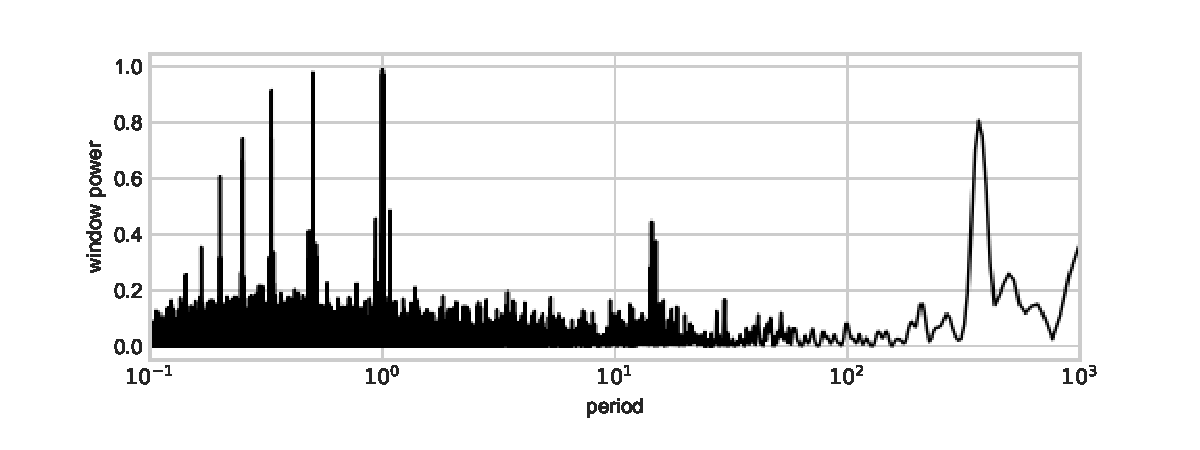
\includegraphics[width=\textwidth]{report/images/chap2_foundations/fig14_LINEAR_window.pdf}
            \end{subfigure}
            \begin{subfigure}{\textwidth}
                \centering
                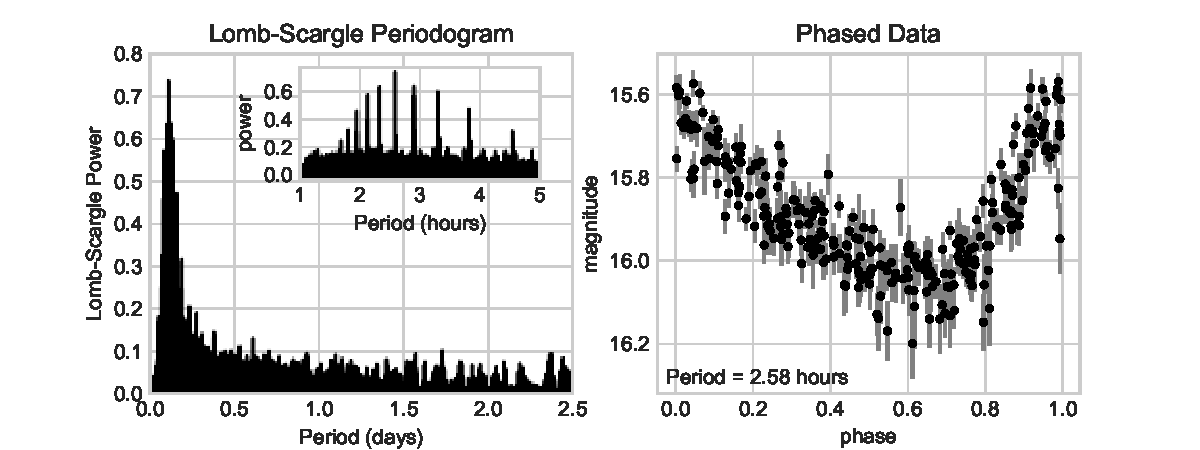
\includegraphics[width=\textwidth]{report/images/chap2_foundations/fig02_LINEAR_PSD.pdf}
                %\vspace{2em}
            \end{subfigure}%
            \caption{???}
            \label{2.4b}
            \end{figure}
            
        \subsection{Other methods}

        
    \section{Distance correlation-based periodograms}

    
        \begin{figure}[H]
        \centering
        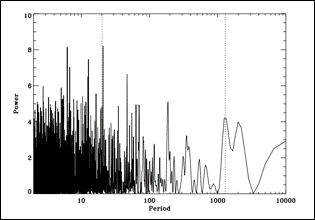
\includegraphics[width=0.5\textwidth]{report/images/chap2_foundations/carolo_2014.png}
        \caption{Caption}
        \label{2.5a}
        \end{figure}
        
        \subsection{Mathematical framework}

                
        \begin{figure}[H]
        \centering
        \begin{subfigure}{.45\textwidth}
            \centering
            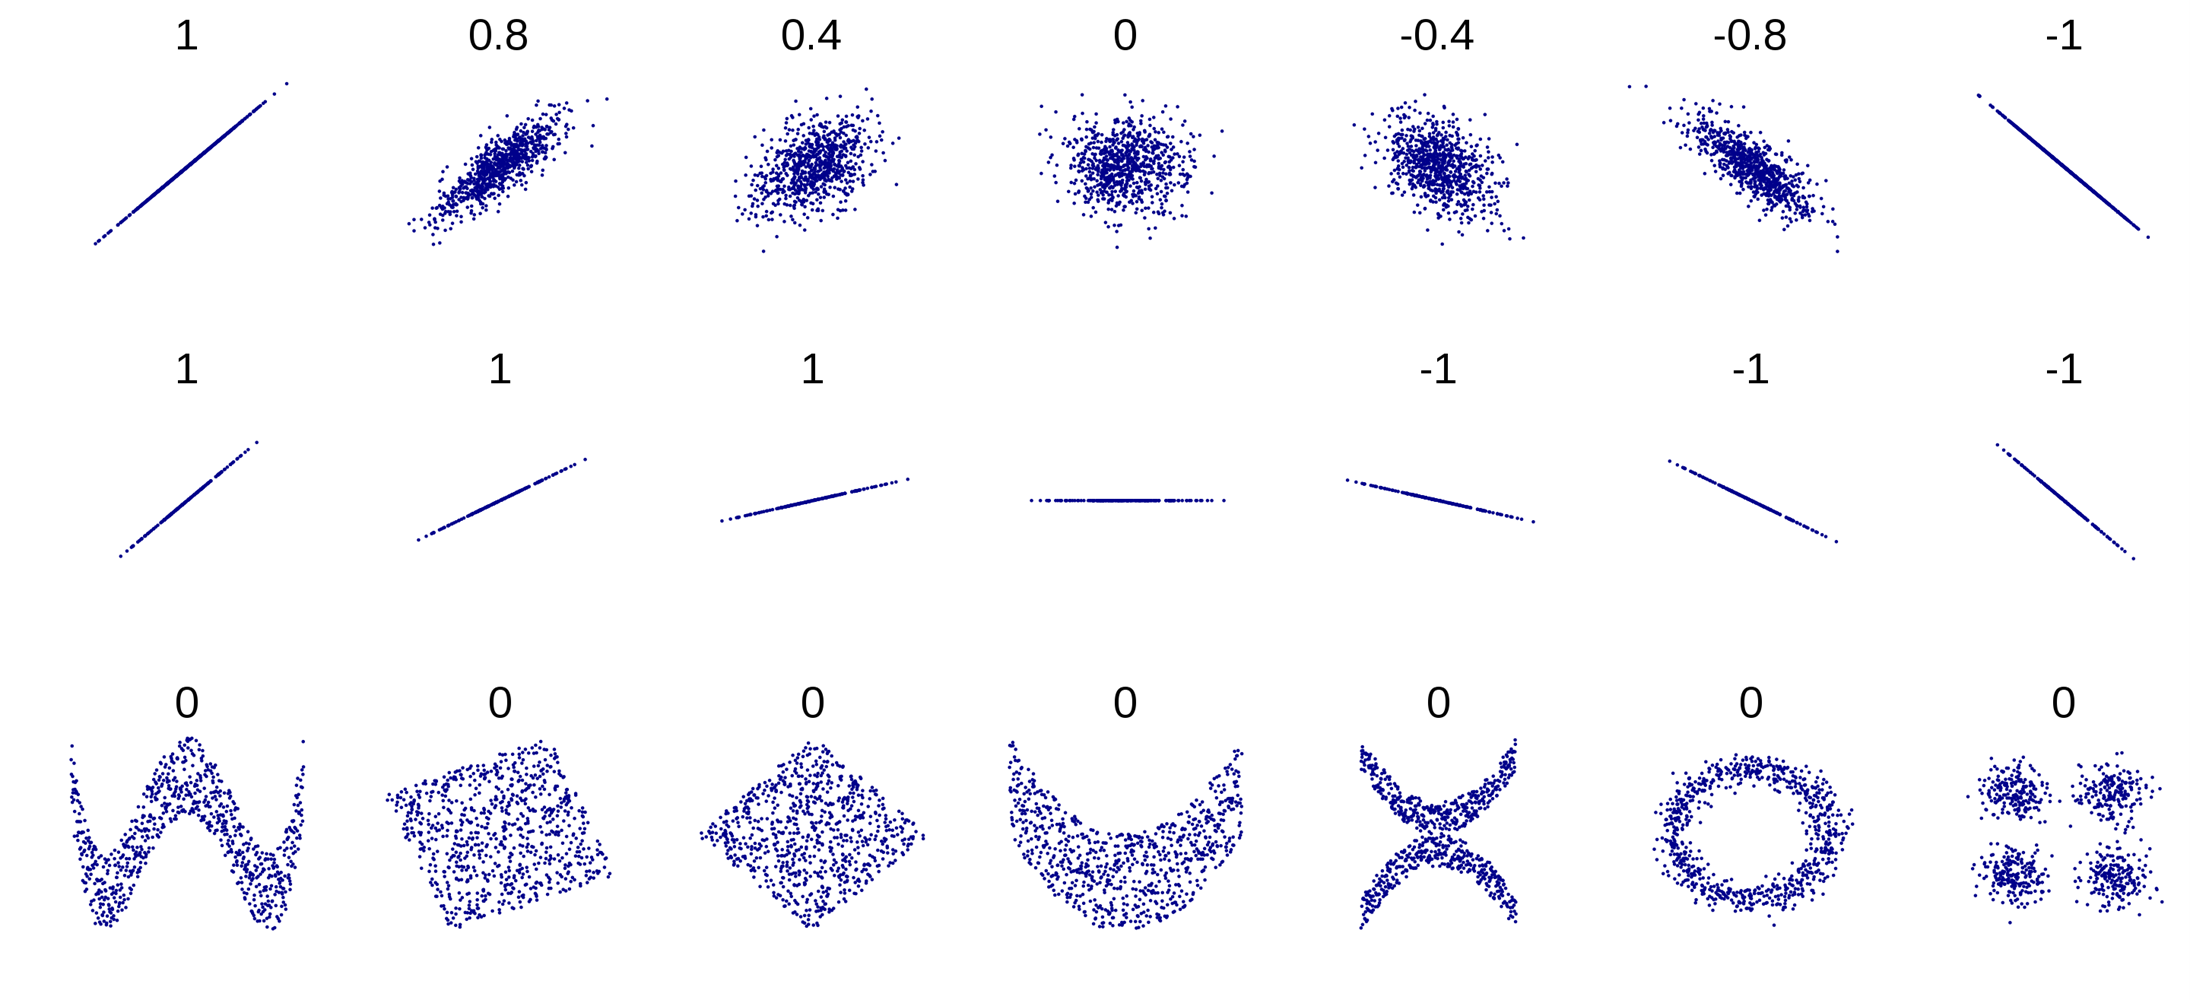
\includegraphics[width=\textwidth]{report/images/chap2_foundations/Correlation_examples2.svg.png}
            \vspace{1em}
        \end{subfigure}%
        \hspace{1em}
        \begin{subfigure}{.45\textwidth}
            \centering
            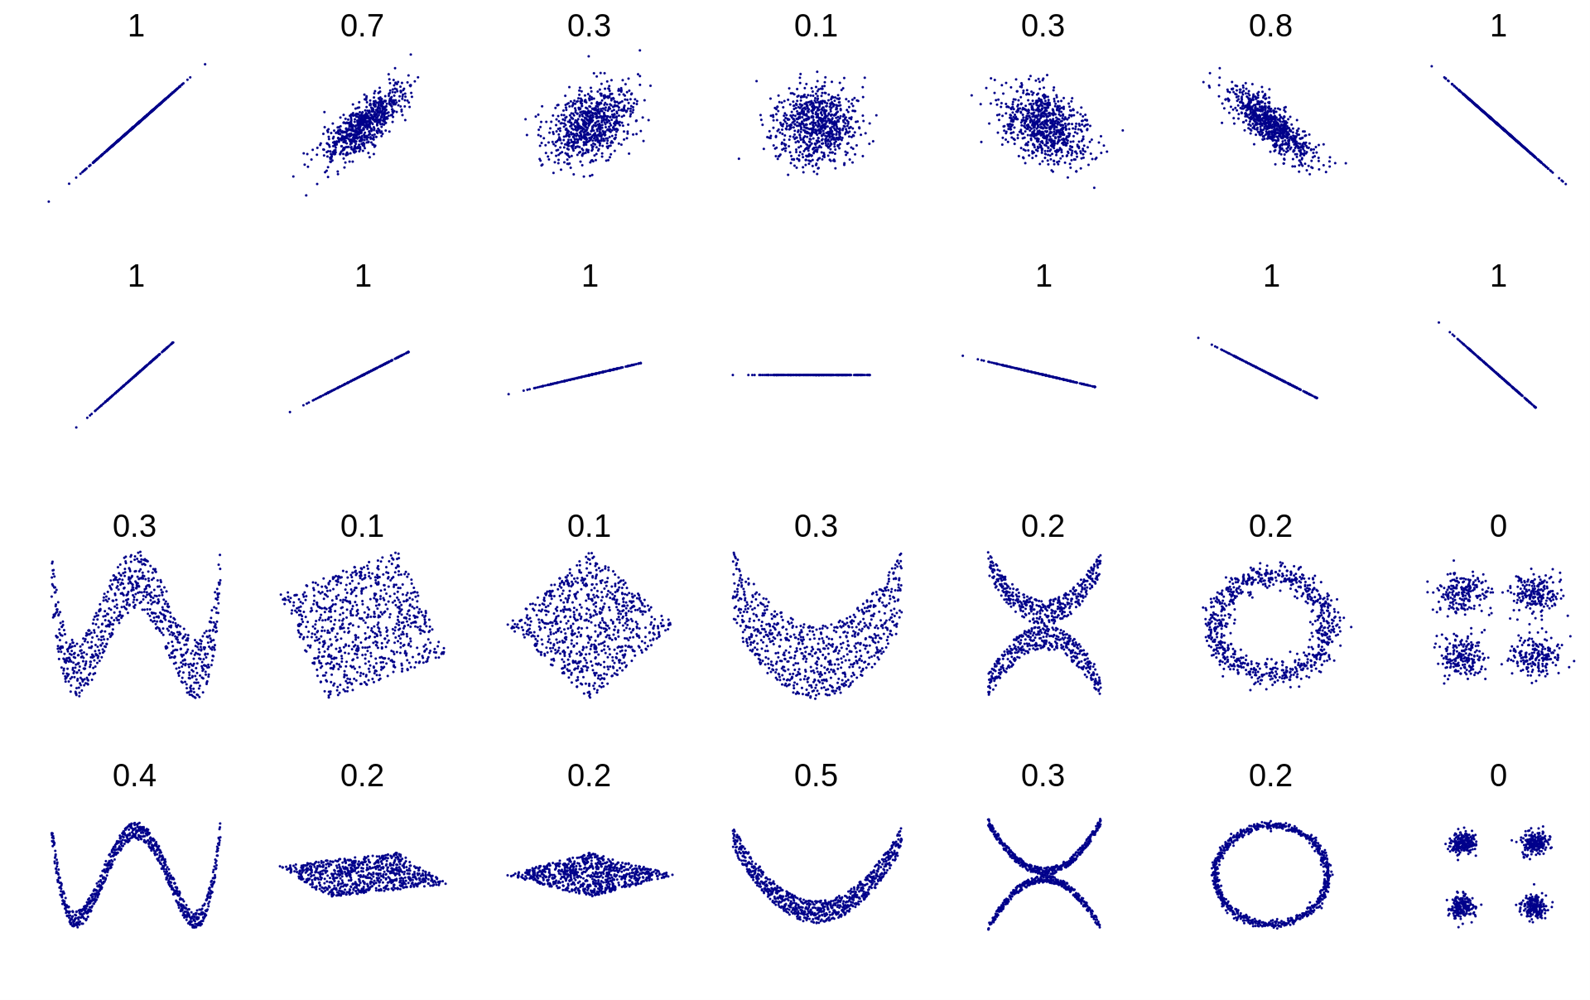
\includegraphics[width=\textwidth]{report/images/chap2_foundations/Distance_Correlation_Examples.svg.png}
        \end{subfigure}
        \caption{???}
        \label{2.5b}
        \end{figure}

        \subsection{A didactic example}

        \begin{figure}[H]
        \centering
        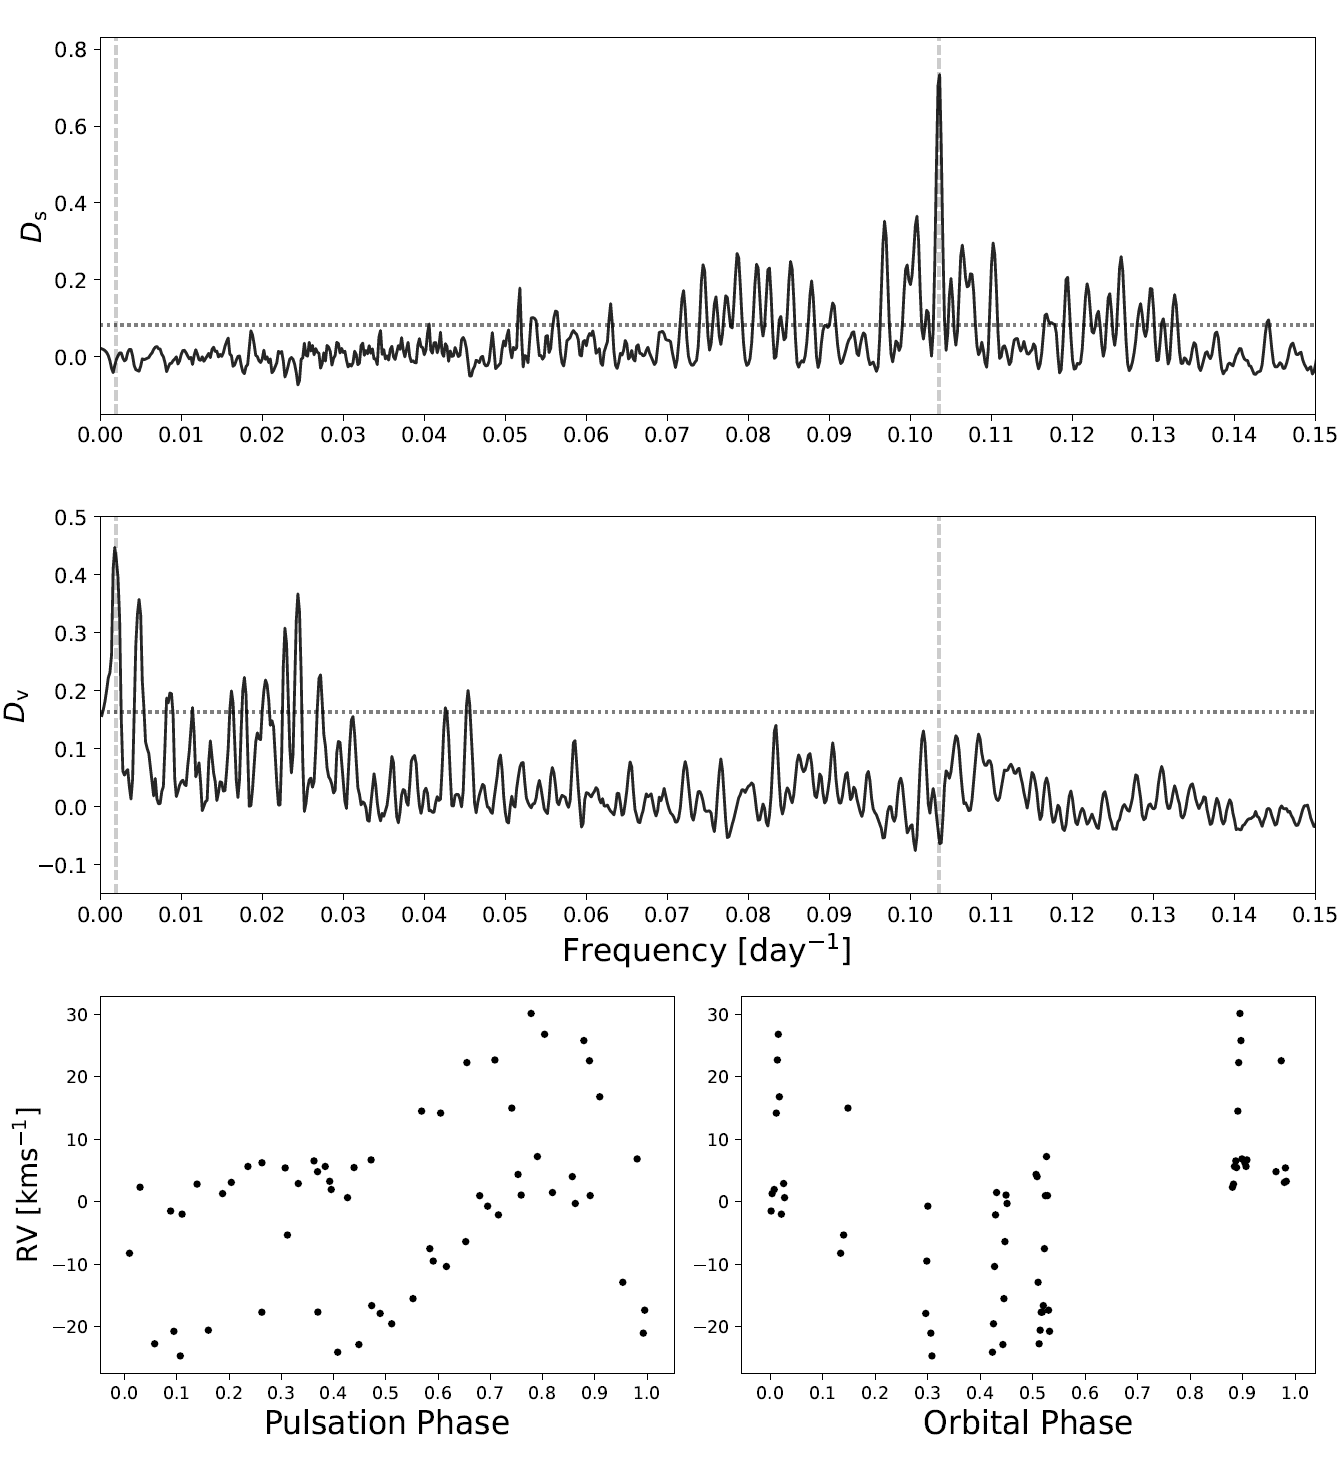
\includegraphics[width=\textwidth]{report/images/chap2_foundations/Smus.png}
        \caption{Caption}
        \label{2.5c}
        \end{figure}

        \begin{figure}[H]
        \centering
        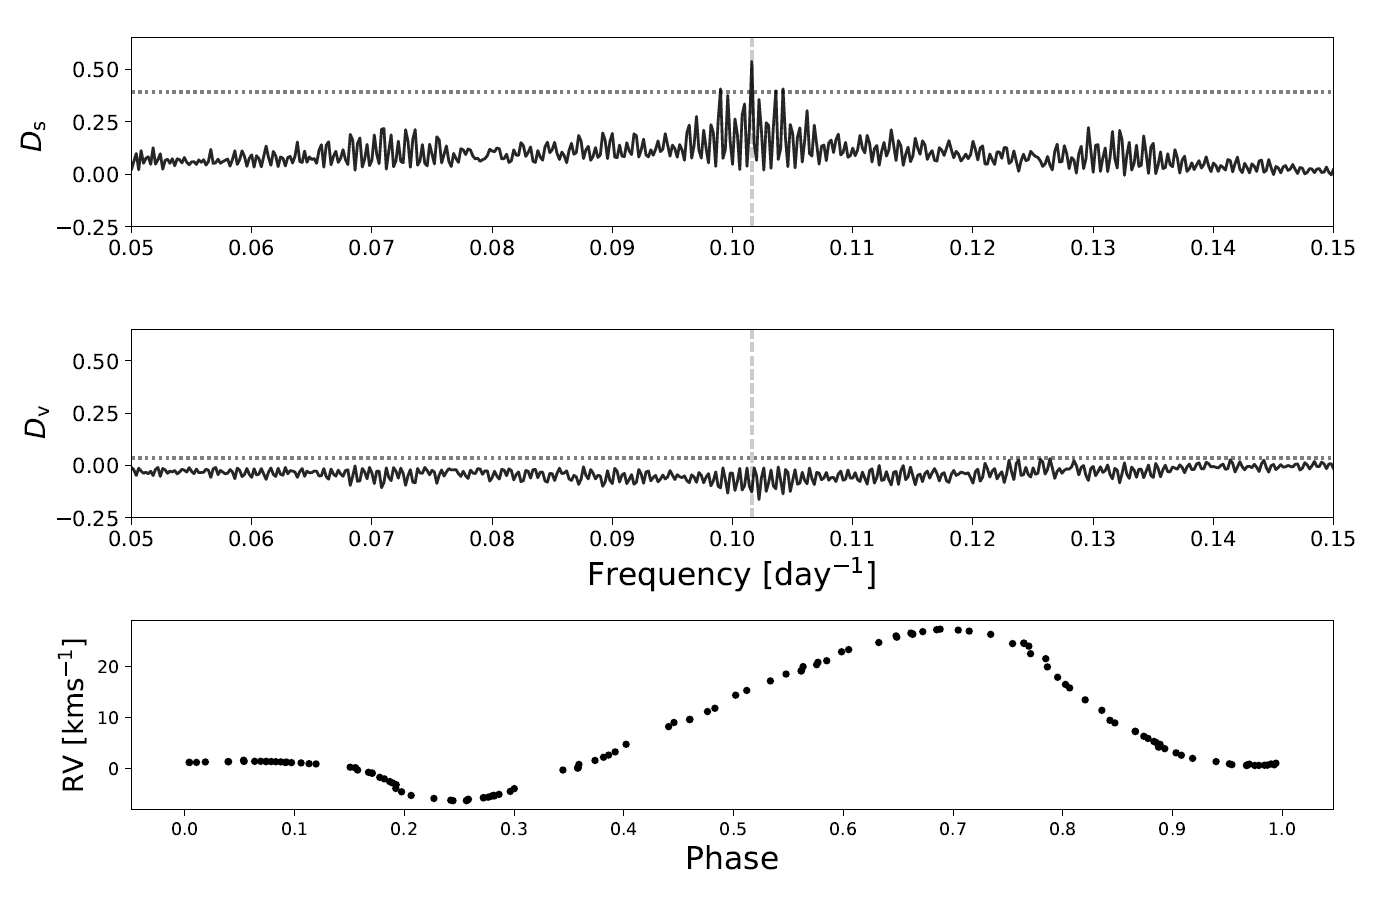
\includegraphics[width=\textwidth]{report/images/chap2_foundations/betador.png}
        \caption{Caption}
        \label{2.5d}
        \end{figure}
%%%%%%%%%%%%%%%%
\chapter{Methodology}
\label{methods}
    %%%%%%%%%%%%%%%%
    \section{Instruments}
    %% Add efficiency of both detectors with respect to wavelength to explain why we choose 5000 rather that 4000 in general and in particular for BG Cru when looking at the second periodicity(why it's bigger).
        \begin{figure}[H]
        \centering
        \begin{subfigure}{.45\textwidth}
            \centering
            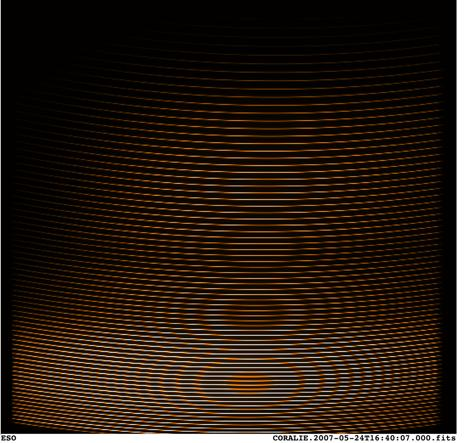
\includegraphics[width=0.8\textwidth]{report/images/chap3_methods/coralie_grating.jpg}
            \vspace{2em}
        \end{subfigure}%
        \hspace{1em}
        \begin{subfigure}{.45\textwidth}
            \centering
            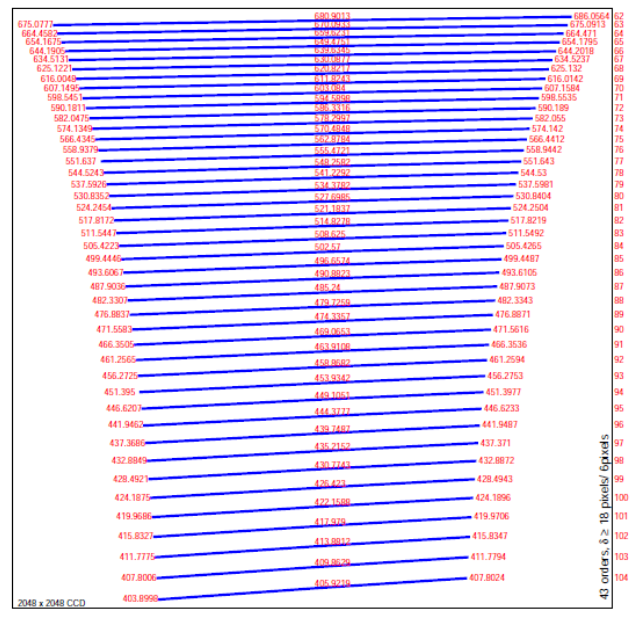
\includegraphics[width=\textwidth]{report/images/chap3_methods/echellogram.png}
        \end{subfigure}
        \caption{???}
        \label{3.1a}
        \end{figure}

        \begin{figure}[H]
        \centering
        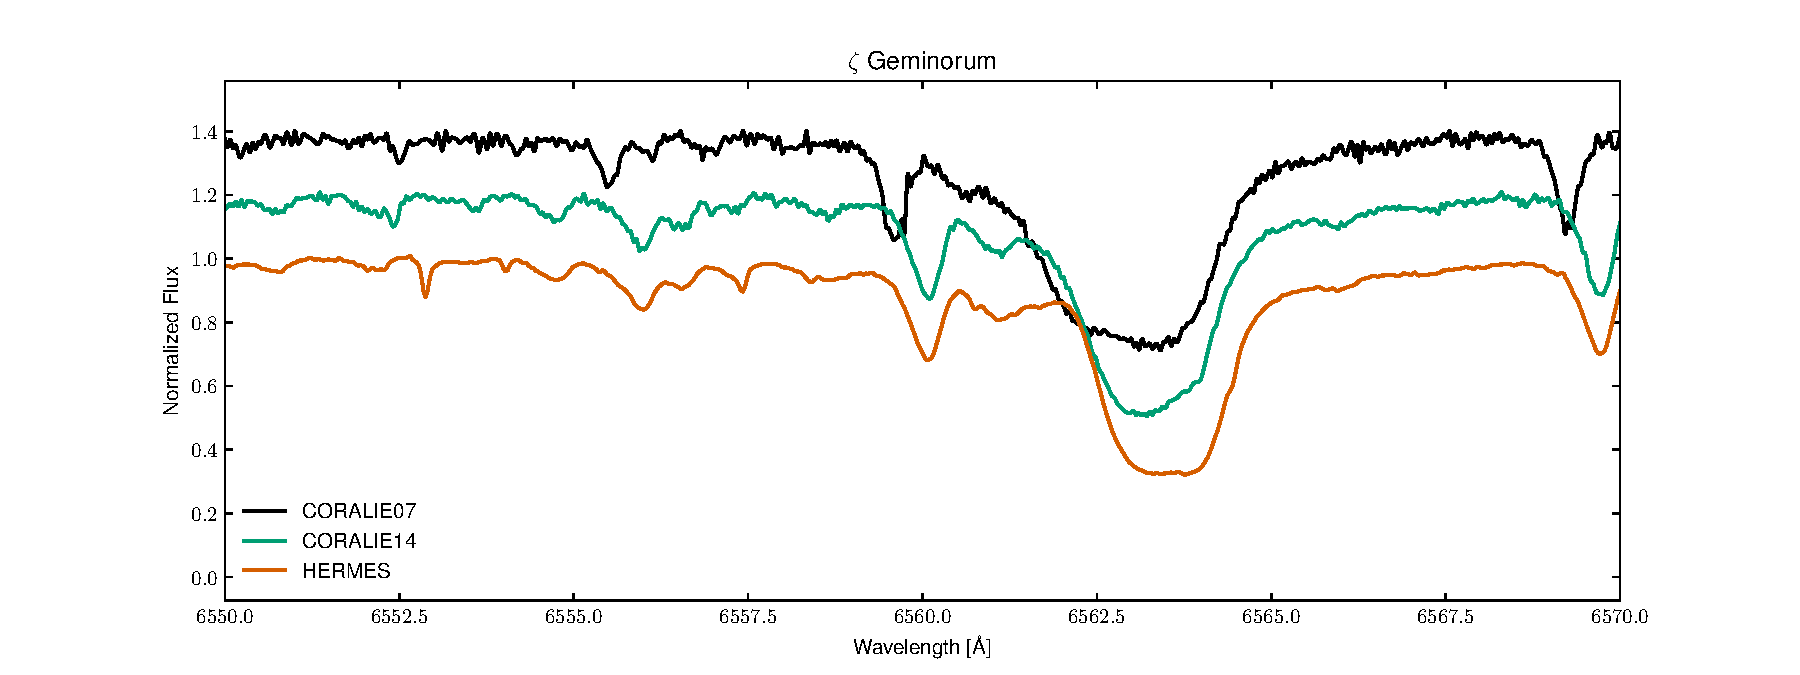
\includegraphics[width=\textwidth]{report/images/chap3_methods/zetgem_hermes_coralie.pdf}
        \caption{Caption}
        \label{3.1b}
        \end{figure}
    
        \subsection{CORALIE}
            \subsubsection{CORALIE07}
            \subsubsection{CORALIE14}
        \subsection{HERMES}
        \begin{figure}[H]
        \centering
        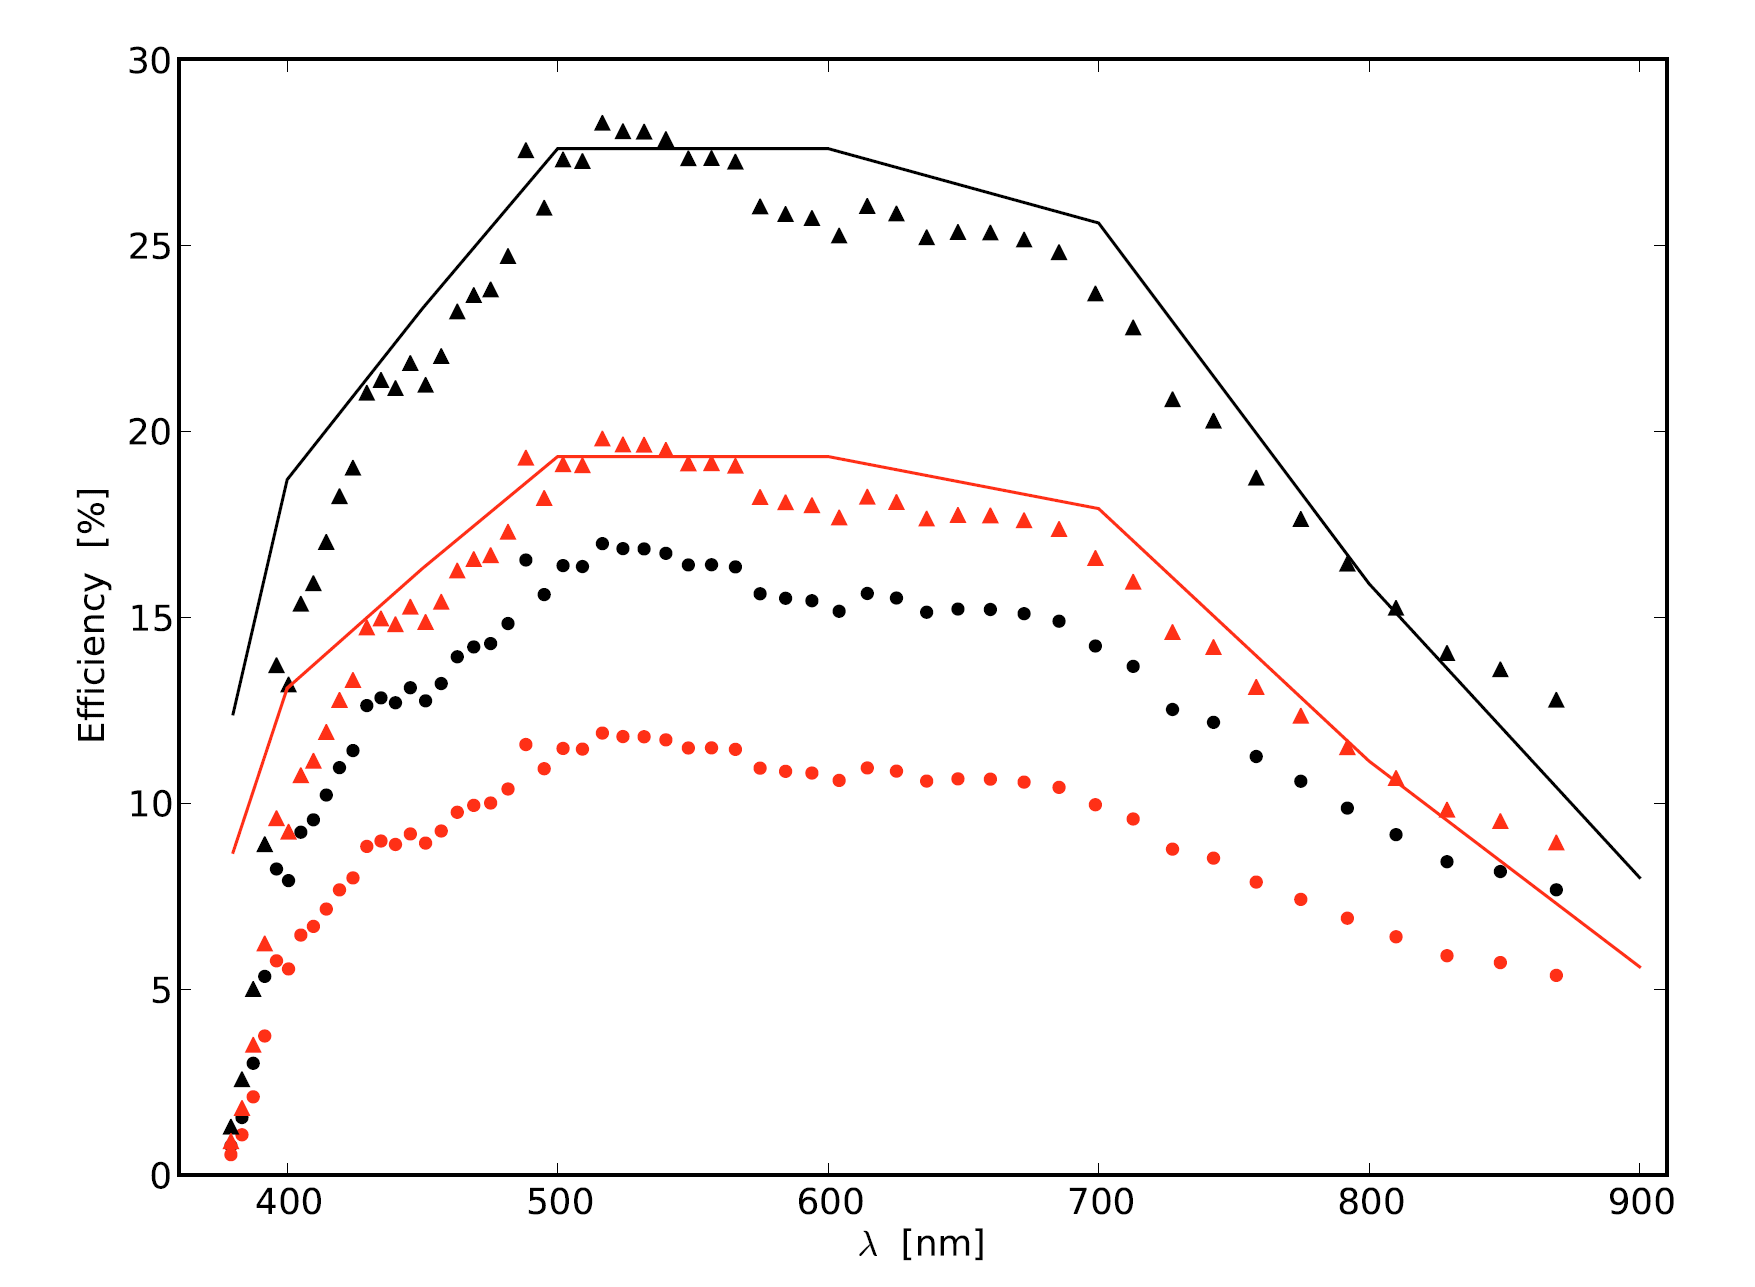
\includegraphics[width=0.6\textwidth]{report/images/chap3_methods/efficiency_hermes.png}
        \caption{Caption}
        \label{3.1c}
        \end{figure}
    \section{Data}
    %say data post and after 2018 for hermes + coralie7 and 14
    \subsection{Spectra}
    \subsection{Radial Velocities}
    \section{The SPARTA package}
    %Explain how it works step by step
    \subsection{Spectrum preprocessing}

        \begin{figure}[H]
        \centering
        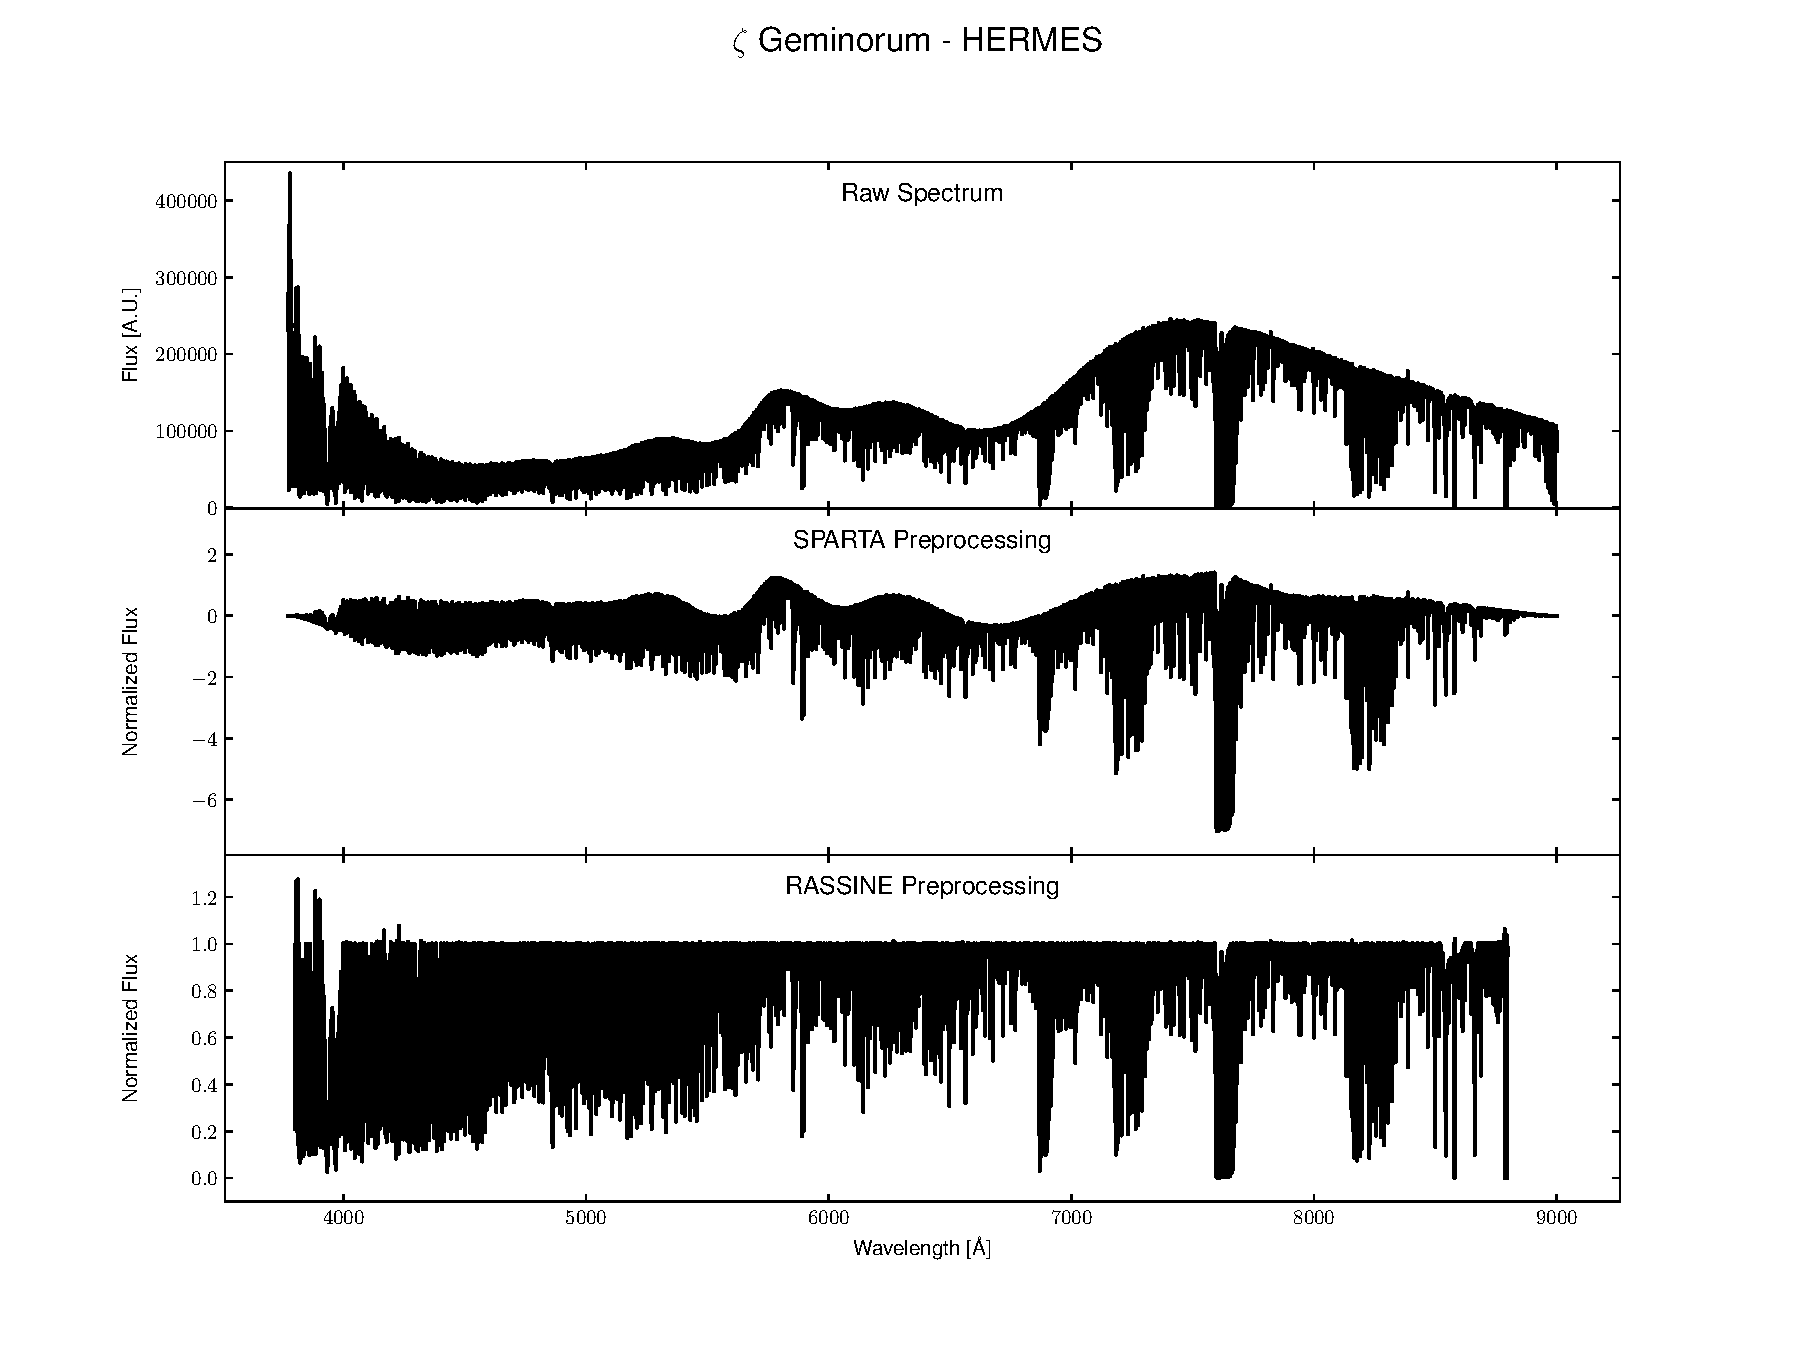
\includegraphics[width=\textwidth]{report/images/chap3_methods/zetgem_preprocessing_hermes.pdf}
        \caption{Caption}
        \label{3.3a}
        \end{figure}

        \begin{figure}[H]
        \centering
        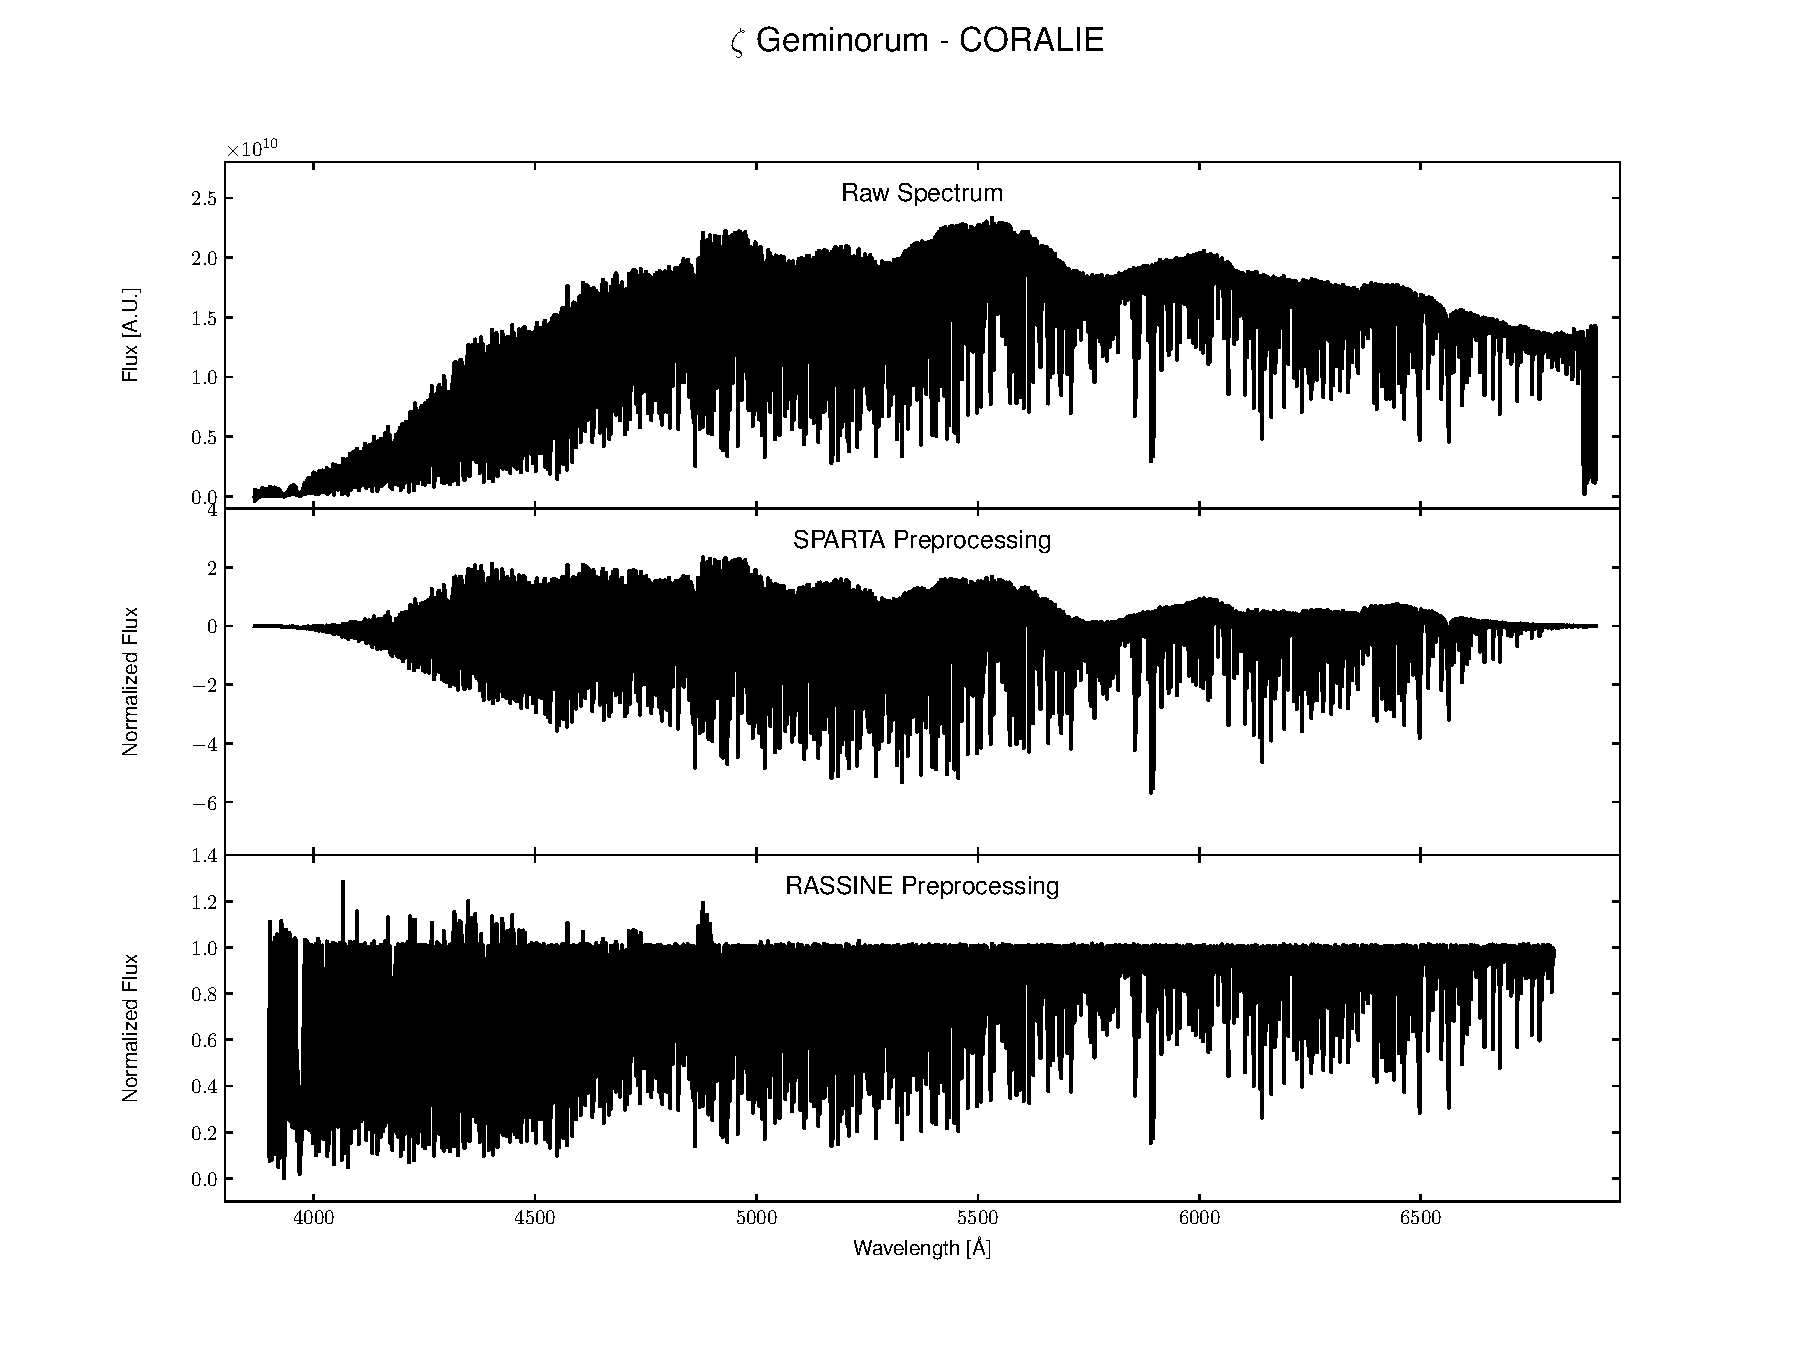
\includegraphics[width=\textwidth]{report/images/chap3_methods/zetgem_preprocessing_coralie14.pdf}
        \caption{Caption}
        \label{3.3b}
        \end{figure}
    
    \subsubsection{The RASSINE method}
    %explain why you use continuum linear and not cubic
    \section{Asserting a peak's statistical significance}
    %explain that in gls and non uniformly sampled periodograms in general, the harmonics and aliases are less power than in uniformly sampled data.

        \begin{figure}[H]
        \centering
        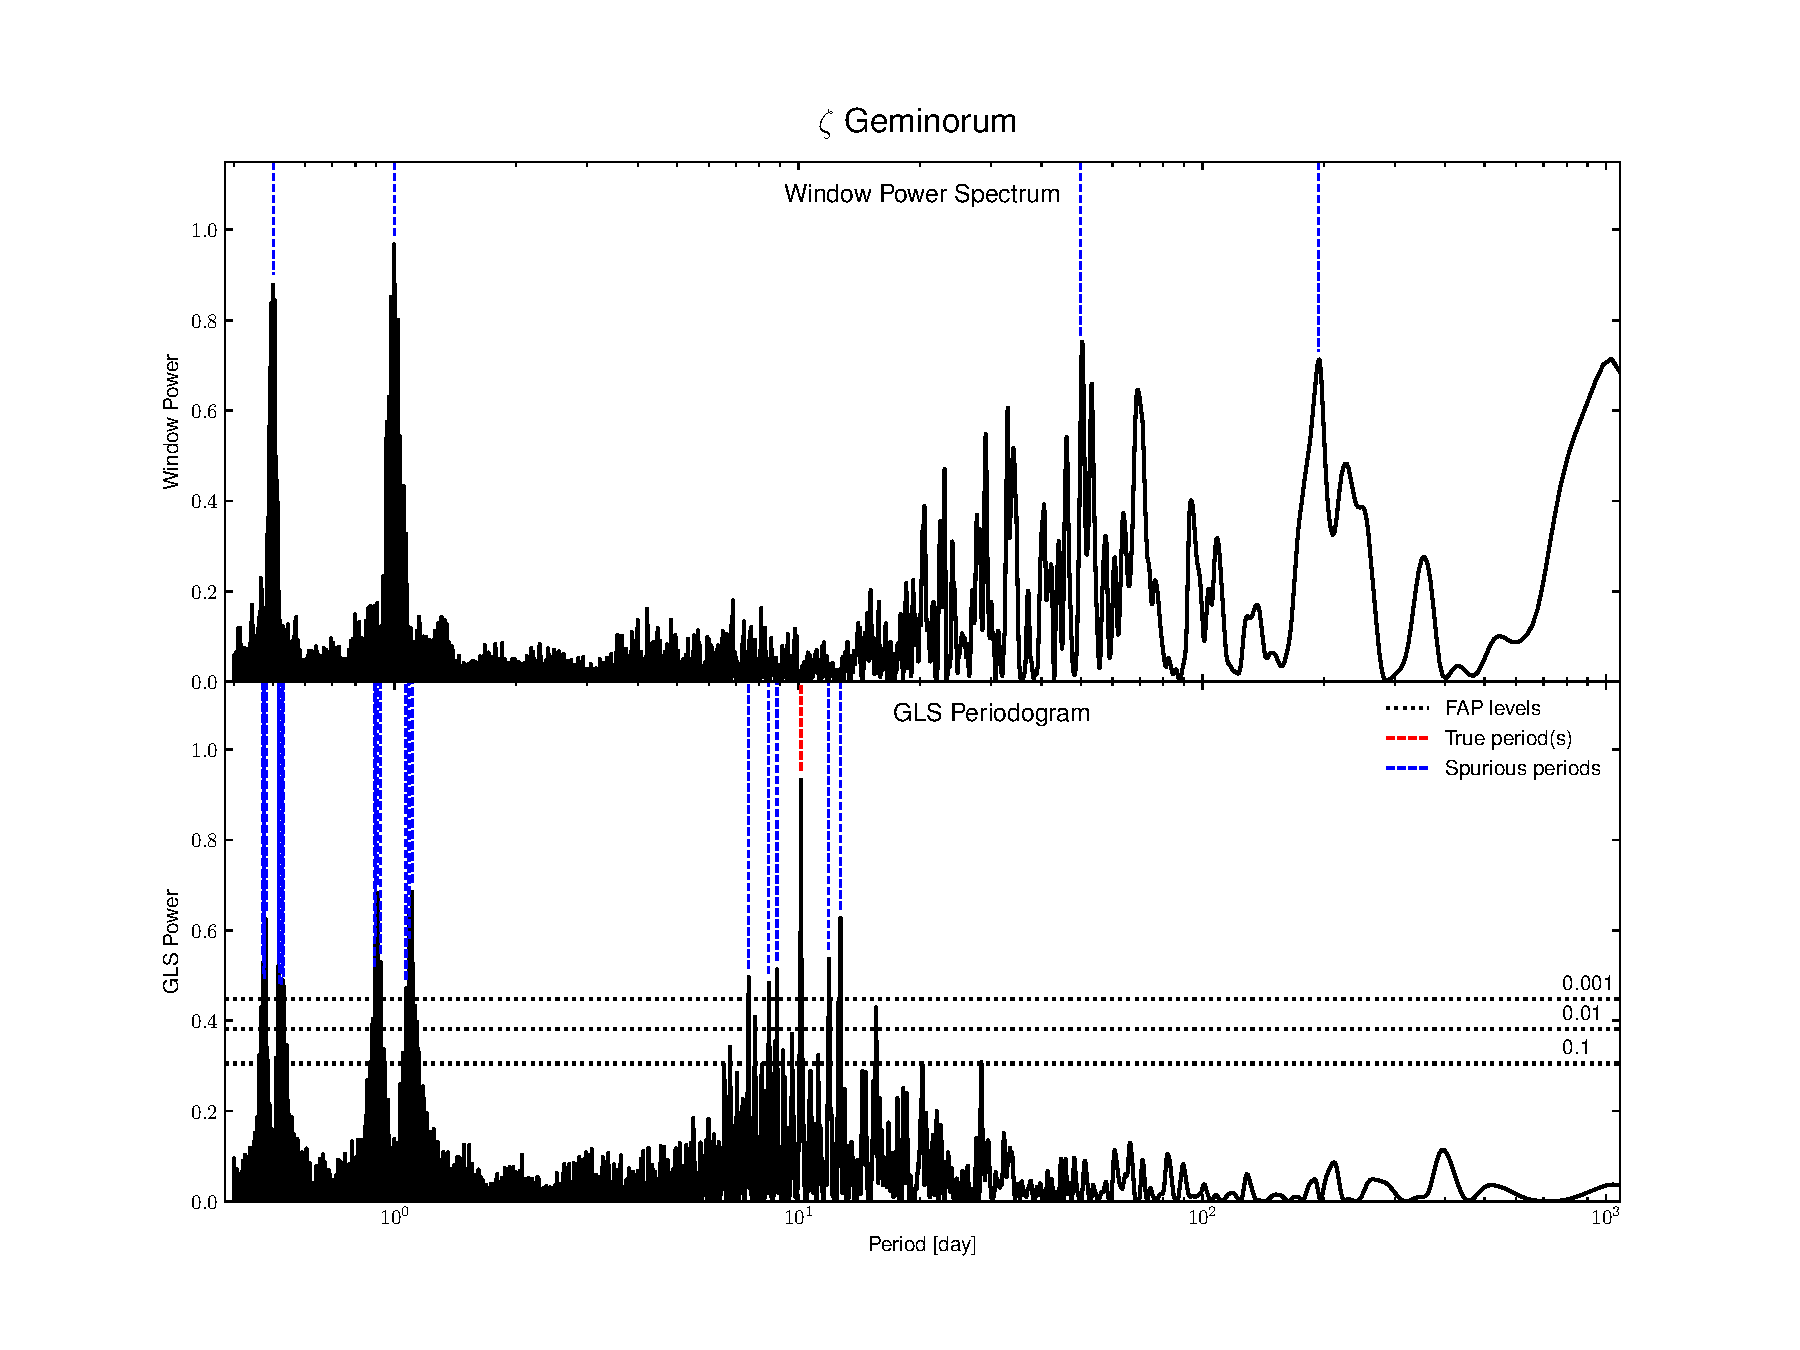
\includegraphics[width=\textwidth]{report/images/chap3_methods/windows_examples.pdf}
        \caption{Caption}
        \label{3.4a}
        \end{figure}
    \subsection{Window functions}
    \subsection{Failure modes: harmonics and aliases}
    \subsection{False-alarm rates and p-values}
as
%%%%%%%%%%%%%%%%%%%%%%%%
\chapter{Chasing systematics}
\label{resultsa}
%%%%%%%%%%%%%%%%%%%%%%%%
%say that you first did some tests with different wavelength ranges and that you saw weird things
    \section{Impact of Earth's atmosphere and the interstellar medium on the spectra}
    \begin{figure}[H]
        \centering
        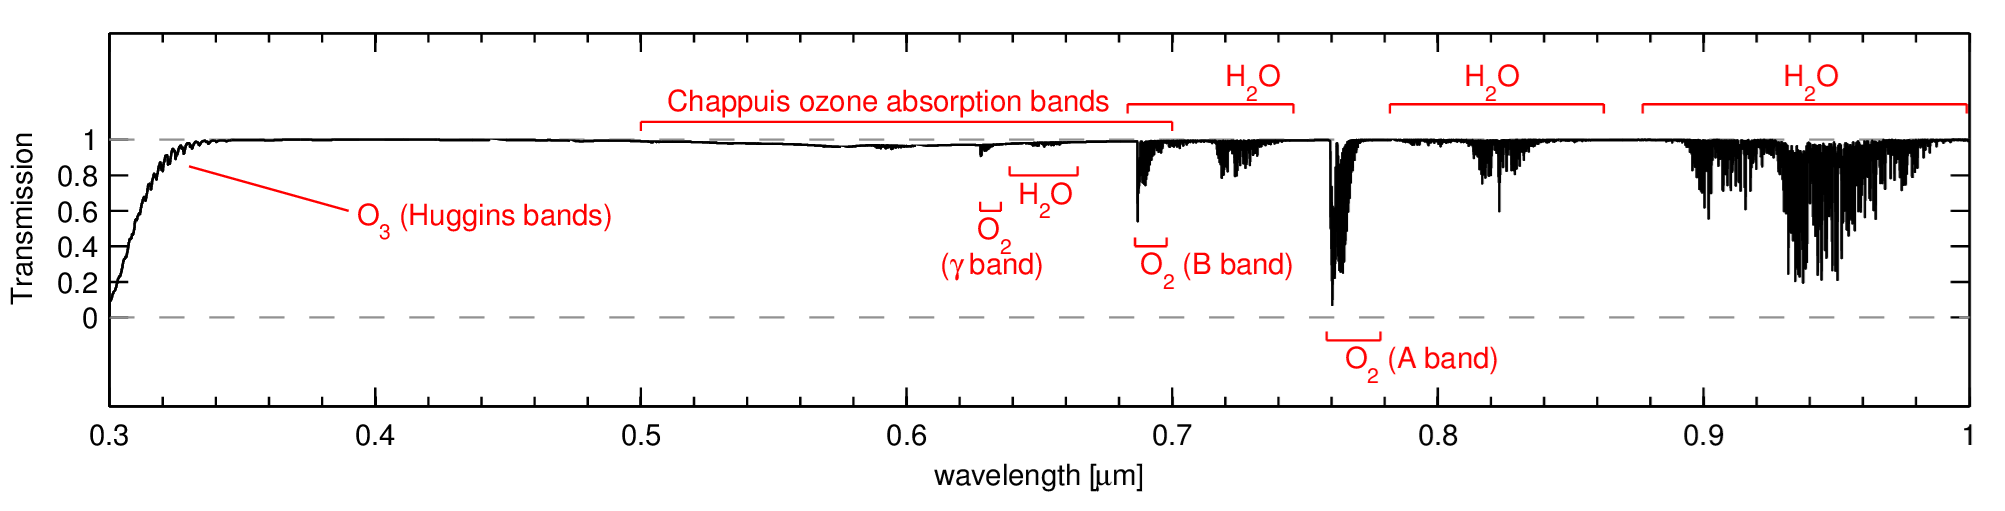
\includegraphics[width=\textwidth]{report/images/chap4_results/paranal_smette.png}
        \caption{Caption}
        \label{4.1a}
    \end{figure}
        \subsection{Tellurics}
        %test if by masking tellurics it works
        \subsection{The sodium doublet}
        \subsection{Low-frequency variations and the influence of the wavelength range's size}
        %show comparison of peak power for shape and shift for different sizes using rassine and explain that since rv computed with whole spectrum then the bigger the wavelength range the better the results: the shift is well suppressed(maybe take the ratio of significance between shape and shift to show that it diminishes ? ) -> explain why: rvs are computed using an "averaged" spectral line. So it is an averaged rv. So two things: 1. Using a bigger range means we represent the rv better so the shift is better suppressed. 2. Parts of the spectra represent better the rv in question but that depends ultimately on the star and its own characteristics so there is probably no better range. The best is to have the rv used for the periodogram computed with the same spectra used in the periodogram.
    \section{Upward and downward trends in the partial periodograms}
    %do the fits maybe ? Use polaris and some other less pronounced star as examples. Say that it was already present in SMus
    %this trend makes me wonder if even the bootstrap to compute the fap is relevant.
    %if the number of observations is sufficient, applying rassine corrects the residual trend and it's all good. So basically the trend is due to several factors.
    %%%%%%%%%%%%%%%%%%%%
    %Explain that the dinosaur shapes are maybe some oversampling of the peaks because we have very few observations.
\chapter{Analysis of 15 Cepheids}
\label{resultsb}
    \section{CORALIE07}
    \section{CORALIE14}
    \section{HERMES}




\chapter{Future work}
\label{future}
%three ways of solving the peak rv: either compute new rvs from spectra range used or the other way around, use the max spectra from rv used.-> ask what ranges they use to compute rvs. Or compute rvs differently-> centroid ?

%%%%%%%%%%%%%%%%%%%%
\chapter{Conclusion}
\label{conclusion}
%%%%%%%%%%%%%%%%%%%%

% Talk about wavelets, CLEAN deconvolution, exoplanets, rassine, bg cru, nlogn, rv accuracy, use of the rv computed from the same range as selected etc...

%don't forget to quote numpy, astropy, sparta, rassine etc...

\appendix
\chapter{Appendix}

\cleardoublepage
\phantomsection
\addcontentsline{toc}{chapter}{Bibliography}
\printbibliography

\end{document}